\section{Results}\label{sec:results}
The final binned fit is performed using the $m_T^I$ histogram for all signals and the number of events for the backgrounds.
 
For the OF and SF analysis, for every categories and for every mass point from
200\GeV up to 3\TeV the significance (or p-value da fare) and the 95\% CL
upper exclusion limit are calculated for a width corresponding to the SM width
at each mass.\\

The significance and the p-value are extracted using the ProfileLikelihood method embedded in the CMS Higgs \textit{combine} package. The upper exclusion limit on the signal strength is instead obtained using the Asymptotic method.

\subsection{OF results}\label{sec:results}

In Fig. ~\ref{fig:lim_OF} are shown the CL limit times branching fraction  as a function of the mass for the four jets categories and in Fig.~\ref{fig:lim_OF_comb} the combination of all the categories. The  improvement on the limit respect to 2015 data is around a factor of four.

In Fig.  ~\ref{fig:sig_OF} is shown the significance as a function of the mass for the four jet categories and in Fig. ~\ref{fig:sig_OF_comb} the
combination of all the categories is reported for C'$=$1.


\begin{figure}[htb]
\centering
\subfigure[0 jets]{
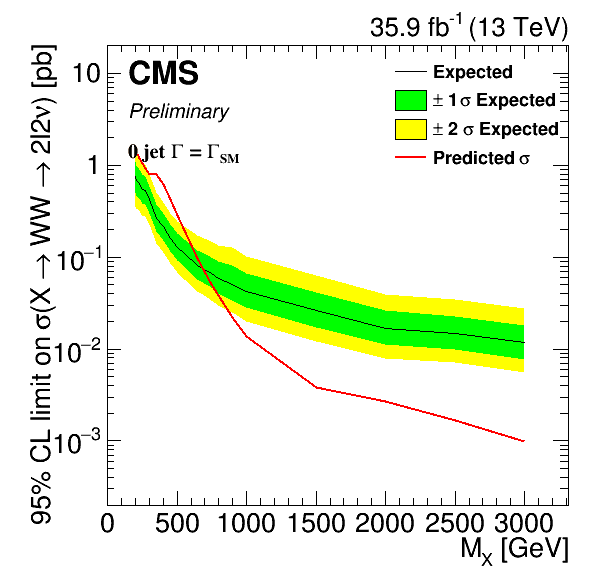
\includegraphics[width=0.45\textwidth]{Figs/Limits_OF/c2_0jet.png}
}
\subfigure[1 jet]{
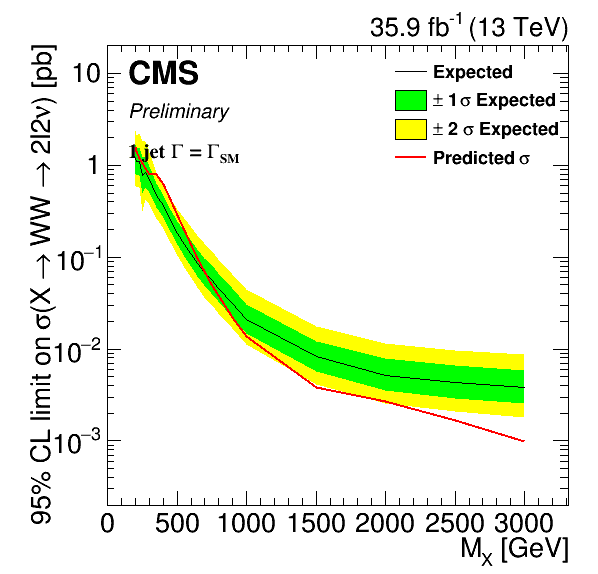
\includegraphics[width=0.45\textwidth]{Figs/Limits_OF/c2_1jet.png}
}
\\
\subfigure[2 jet]{
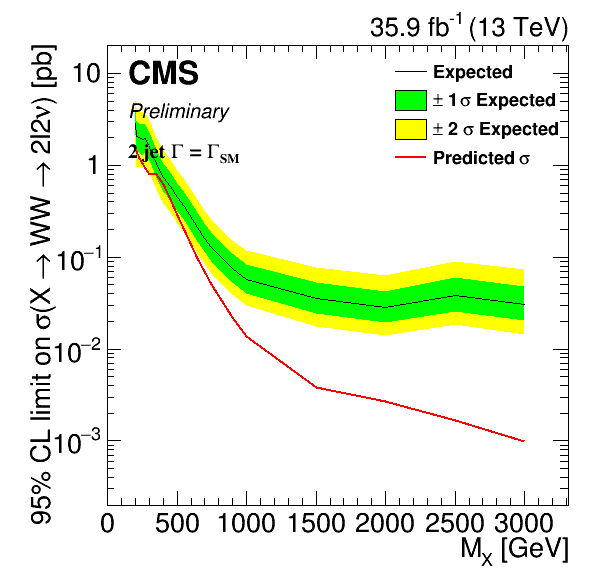
\includegraphics[width=0.45\textwidth]{Figs/Limits_OF/c2_2jet.png}
}
\subfigure[VBF]{
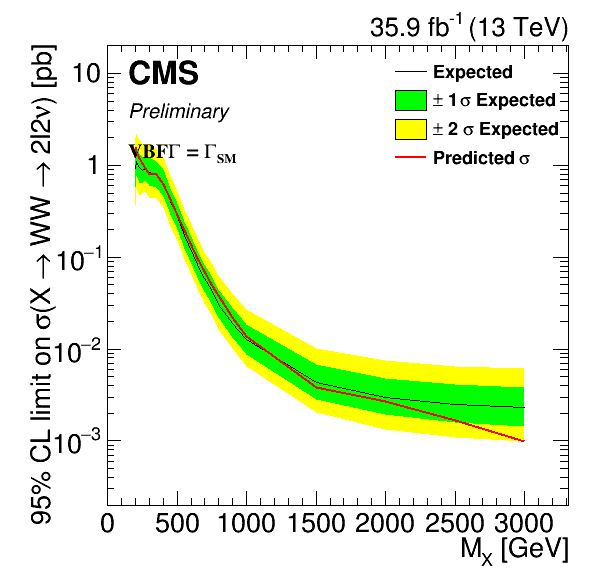
\includegraphics[width=0.45\textwidth]{Figs/Limits_OF/c2_VBF.png}
}


\caption{95$\%$ CL exclusion limits on the production ggH and VBF cross section times branching fraction as a function of the mass for 0 jets, 1 jet, 2jet and VBF categories. The red  line represent the predicted cross-section for EW high mass bosons.}
    \label{fig:lim_OF}
\end{figure}
    


\begin{figure}[htb]
\centering
\subfigure[0 jets]{
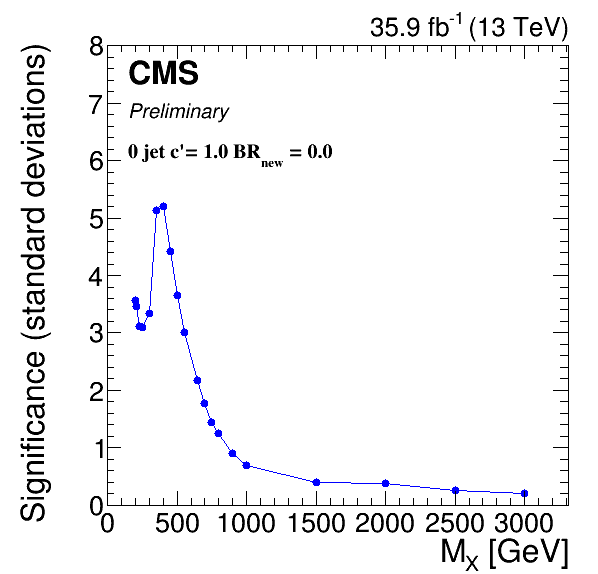
\includegraphics[width=0.45\textwidth]{Figs/Sig_OF/c1_sig_0jet_OF.png}
}
\subfigure[1 jet]{
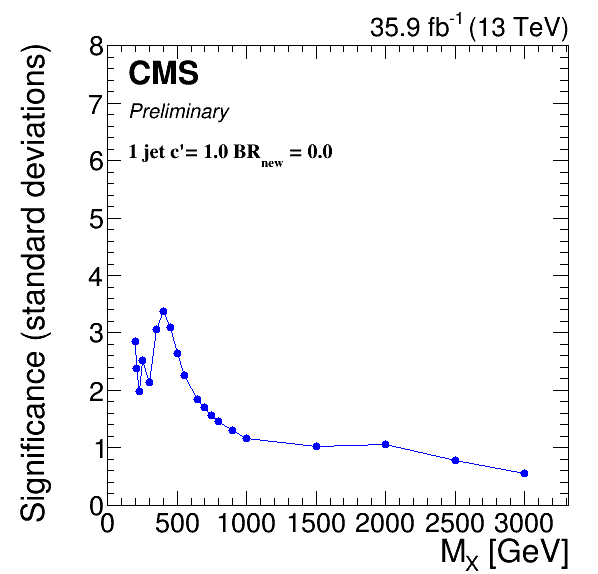
\includegraphics[width=0.45\textwidth]{Figs/Sig_OF/c1_sig_1jet_OF.png}
}
\\
\subfigure[2 jet]{
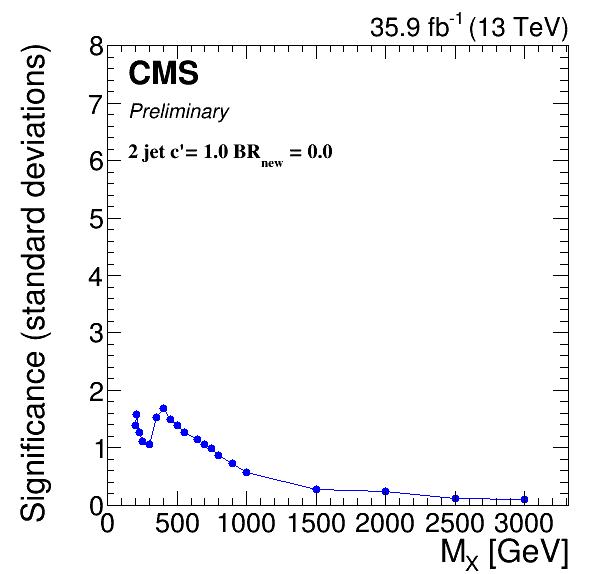
\includegraphics[width=0.45\textwidth]{Figs/Sig_OF/c1_sig_2jet_OF.png}
}
\subfigure[VBF]{
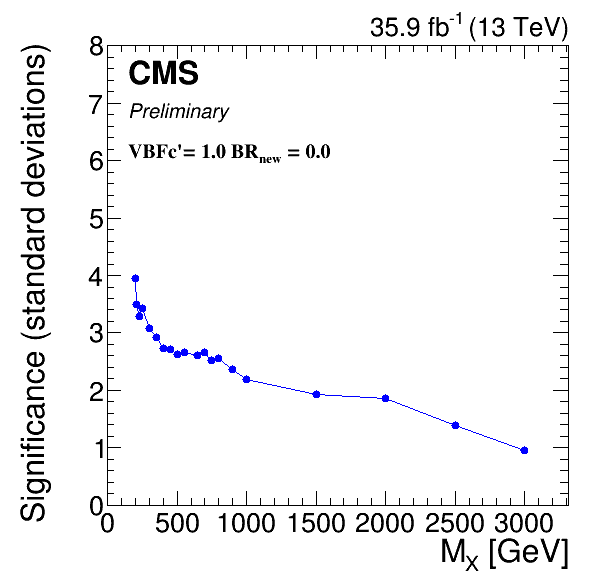
\includegraphics[width=0.45\textwidth]{Figs/Sig_OF/c1_sig_VBF_OF.png}
}


\caption{Significance as a function of the mass for 0 jets, 1 jet, 2jet and VBF categories.}
    \label{fig:sig_OF}
\end{figure}




\begin{figure}[htb]
\centering

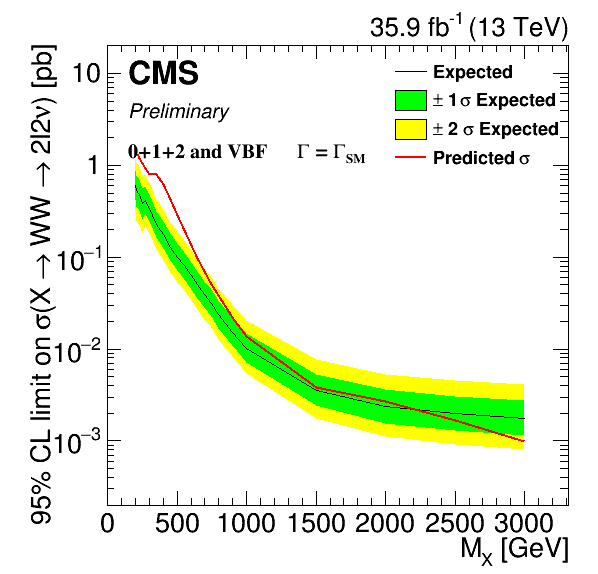
\includegraphics[width=0.65\textwidth]{Figs/Limits_OF/c2_ALL.png}

\caption{95$\%$ CL exclusion limits,  on the production ggH and VBF cross section times branching fraction as a function of the mass for the combination of the {\bf combination} of the four categories in the OF analysis, in the full mass range.   The red  line represent the predicted cross-section for EW high mass bosons.}
    \label{fig:lim_OF_comb}
\end{figure}
    


\begin{figure}[htb]
\centering

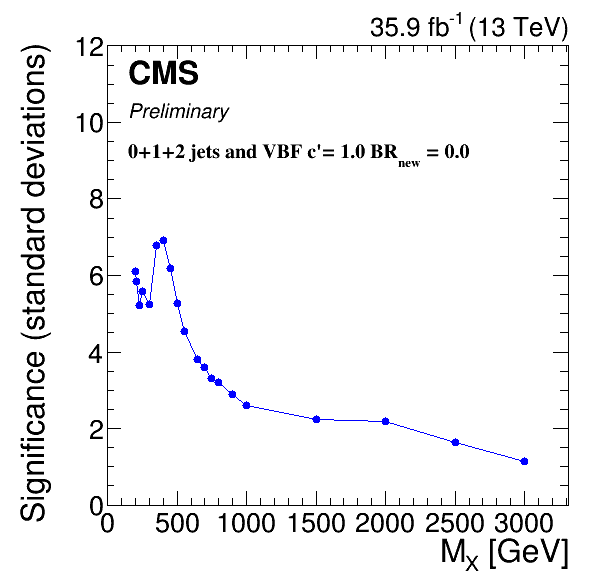
\includegraphics[width=0.65\textwidth]{Figs/Sig_OF/c1_sig_comb_OF.png}

\caption{Combined significance as a function of the mass.}
    \label{fig:sig_OF_comb}
\end{figure}



\newpage
\clearpage 
\subsection{SF results}\label{sec:results}

In Figs ~\ref{fig:lim_SF} are shown the CL limit times branching fraction  as a function of the mass for the same flavour in VBF category for ee and $\mu \mu$ and their combination,  Fig ~\ref{fig:lim_SF_comb}. The limit obtained with the combination of ee and $\mu \mu$ categories, results a bit worse than the 
corresponding limit in the opposite-flavour VBF analysis, Fig. ~\ref{fig:lim_OF} \textit{d}. 
This is understood as due to the greater amount of backgrounds (produced by the Z boson) in the SF analysis.\\

In Fig.  ~\ref{fig:sig_SF} is shown the significance as a function of the mass for the four jet categories and in Fig. ~\ref{fig:sig_SF_comb} the
combination of all the categories is reported for C'$=$1.

\begin{figure}[htb]
\centering
\subfigure[ee]{
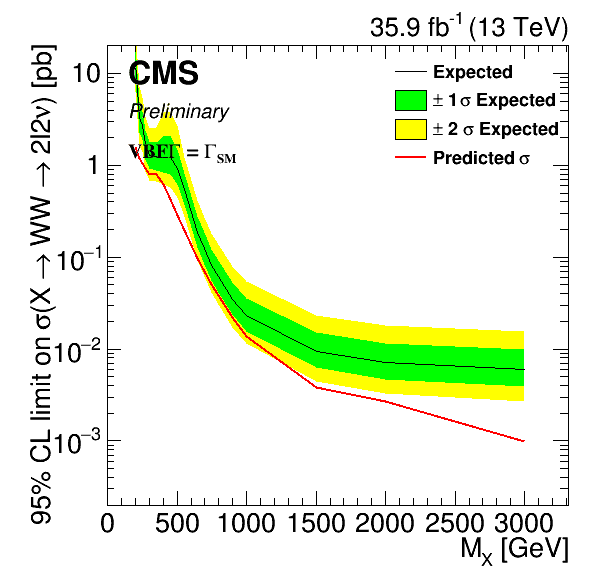
\includegraphics[width=0.45\textwidth]{Figs/Limits_SF/c2_ee.png}
}
\subfigure[$\mu \mu$]{
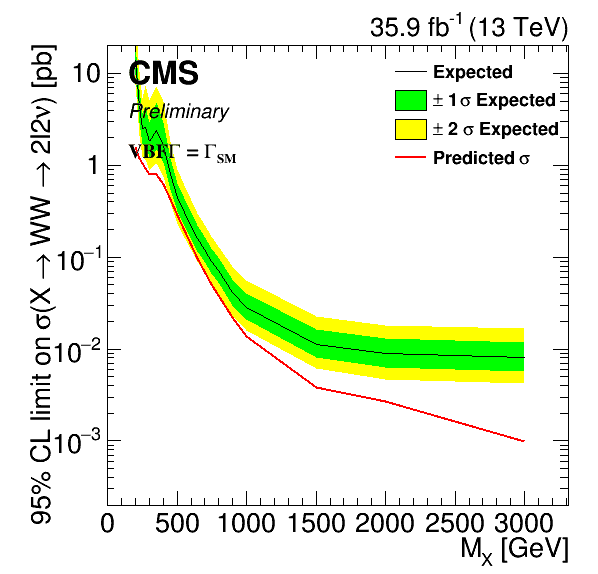
\includegraphics[width=0.45\textwidth]{Figs/Limits_SF/c2_mm.png}
}

\caption{95$\%$ CL exclusion limits, on the production ggH and VBF cross section times branching fraction as a function of the mass for VBF category for ee and $\mu \mu$.  The red  line represent the predicted cross-section for EW high mass bosons.}
    \label{fig:lim_SF}
\end{figure}
    

\begin{figure}[htb]
\centering
\subfigure[ee]{
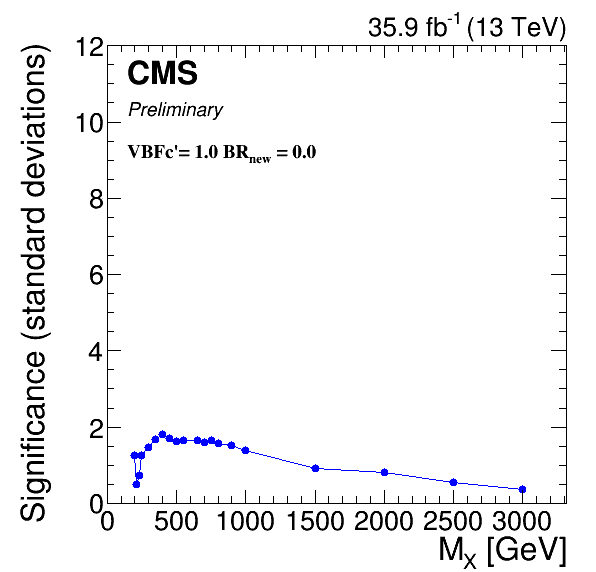
\includegraphics[width=0.45\textwidth]{Figs/Sig_SF/c1_SF_ee_sig.png}
}
\subfigure[$\mu \mu$]{
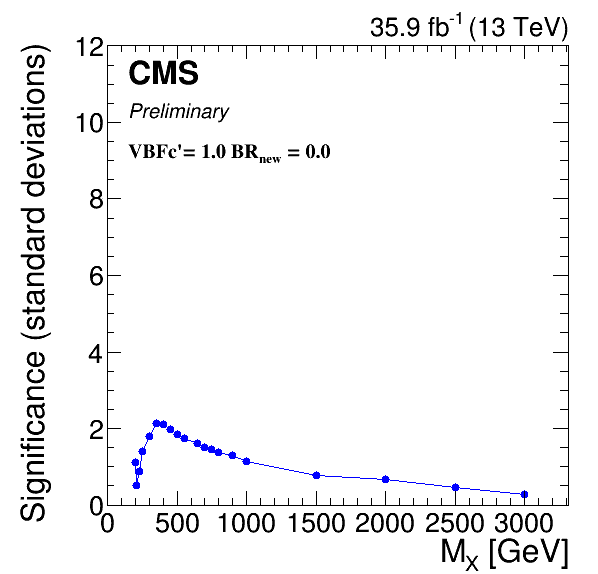
\includegraphics[width=0.45\textwidth]{Figs/Sig_SF/c1_SF_mm_sig.png}
}

\caption{Significance as a function of the mass for ee and $\mu \mu$ categories.}
    \label{fig:sig_SF}
\end{figure}
    


\begin{figure}[htb]
\centering
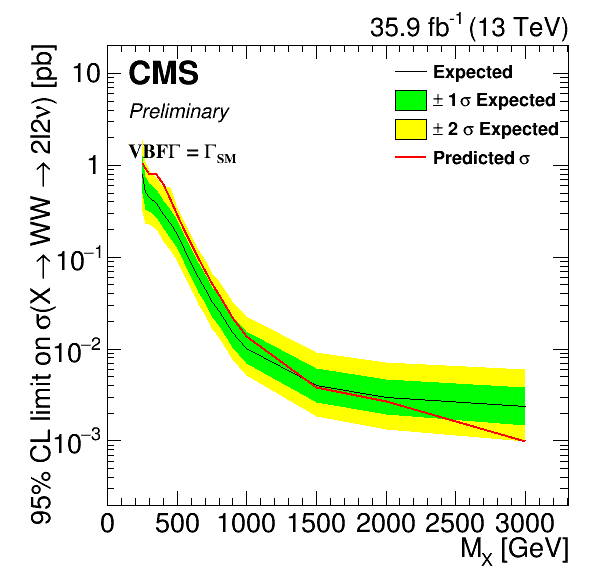
\includegraphics[width=0.65\textwidth]{Figs/Limits_SF/c2_comb.png}
\caption{95$\%$ CL exclusion limits,  on the production ggH and VBF cross section times branching fraction as a function of the mass for the { \bf combination} of the two categories in SF analysis, in the full mass range.   The red  line represent the predicted cross-section for EW high mass bosons.}
    \label{fig:sig_SF_comb}
\end{figure}




\begin{figure}[htb]
\centering
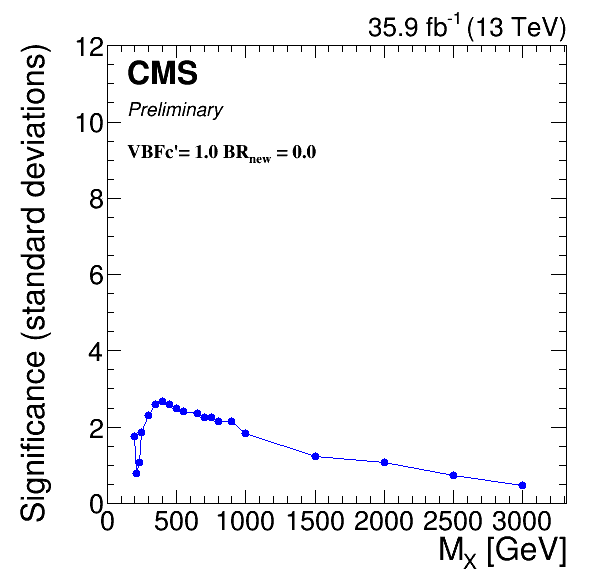
\includegraphics[width=0.65\textwidth]{Figs/Sig_SF/c1_SF_com_sig.png}
\caption{Combined significance as a function of the mass in the OF analysis.}
    \label{fig:sig_SF_comb}
\end{figure}


\newpage
\clearpage

\subsection{Combination}

The expected final limit from the combination of the OF and SF analysis are shown in fig. \ref{fig:lim_OFSF_comb}. 
This limit represent a 	considerable improvement respect to the high mass search done with 2015 data and the expected limits is compatible with the ATLAS results for a similar analysis (CERN-EP-2017-214; arXiv:1710.01123).\\

In Fig.\ref{fig:sig_OFSF_comb} is shown the significance as a function of the mass for the combination of OF and SF analysis.

\begin{figure}[htb]
\centering
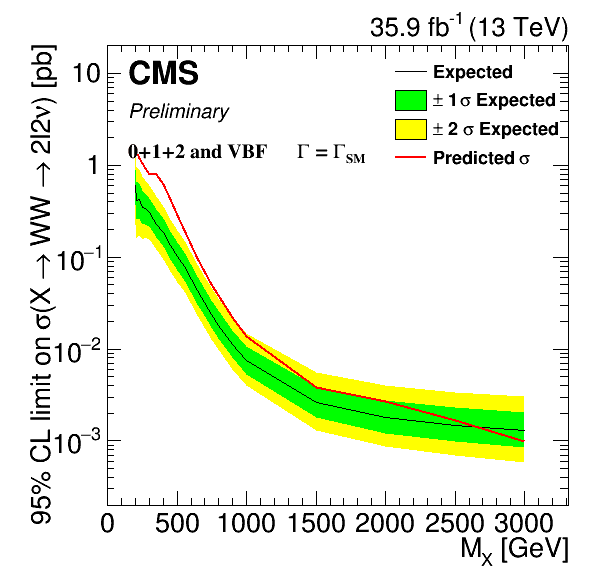
\includegraphics[width=0.65\textwidth]{Figs/Final_comb/c2_OS_comb.png}
\caption{95$\%$ CL exclusion limits,  on the production ggH and VBF cross section times branching fraction as a function of the mass for the { \bf combination} of the two analysis OF and SF, in the full mass range.   The red  line represent the predicted cross-section for EW high mass bosons.}
    \label{fig:lim_OFSF_comb}
\end{figure}


\begin{figure}[htb]
\centering
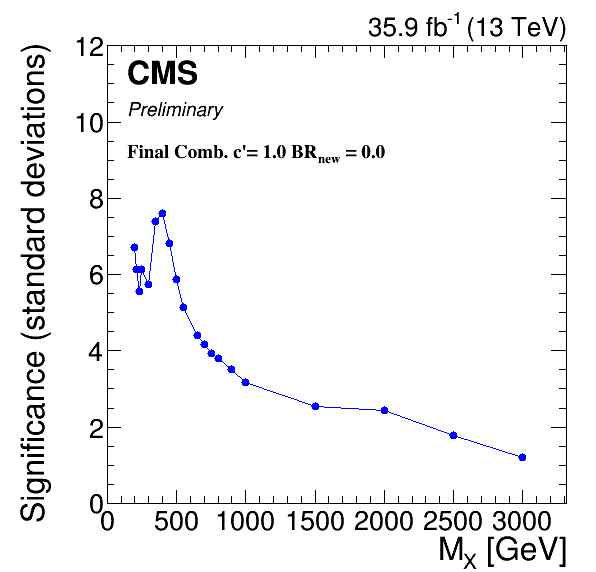
\includegraphics[width=0.65\textwidth]{Figs/Final_comb/c1_sig_OS_comb.png}
\caption{Combined significance as a function of the mass in the OF analysis.}
    \label{fig:sig_OFSF_comb}
\end{figure}

\newpage


\subsection{Limits with different VFB fration}
The production of the X resonance has been considered to be either in gluon gluon fusion and in vector boson fusion with the assumption of the SM fraction. 
However a scan of the fraction of VBF mechanism production ($f_{VBF}$) is performed  to evaluate the  upper limits. So the parameter ($f_{VBF}$), is the fraction of the EW production cross section with respect to the total cross section and the gluon fusion cross section is $\sigma_X \times ( 1 − f_{VBF} )$ .
Three different values of $f_{VBF}$ are studied: $f_{VBF}$ free to floating, $f_{VBF}=0$ and $f_{VBF}=1$. The upper limits for three cases are shown 
in Fig. ~\ref{fig:UL_fvbf} for the combination of the opposite and same flavour analysis.

In the Tab. \ref{tab:UL_ff},  \ref{tab:UL_f1} and \ref{tab:UL_f0} the observed and expected limits values for three masses points (300 GeV, 700 GeV and 1500 GeV) are shown.



\begin{figure}[htb]
\centering

\subfigure[Free to floating]{
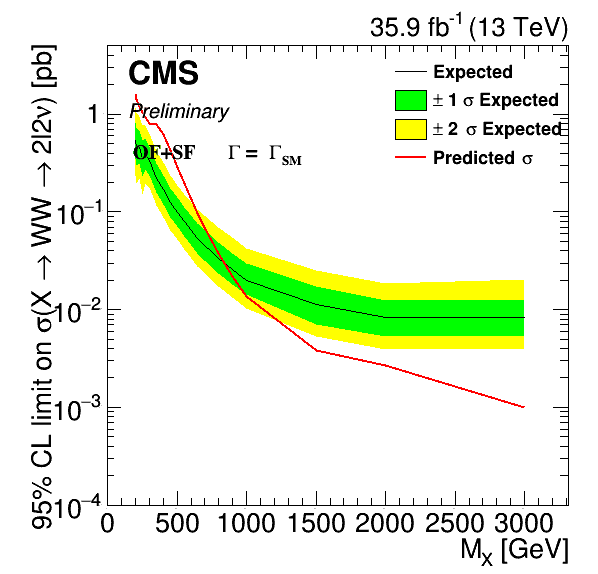
\includegraphics[width=0.45\textwidth]{Figs/Limits_fVBF/c2_floating.png}
}
\subfigure[$f_{VBF}=0$]{
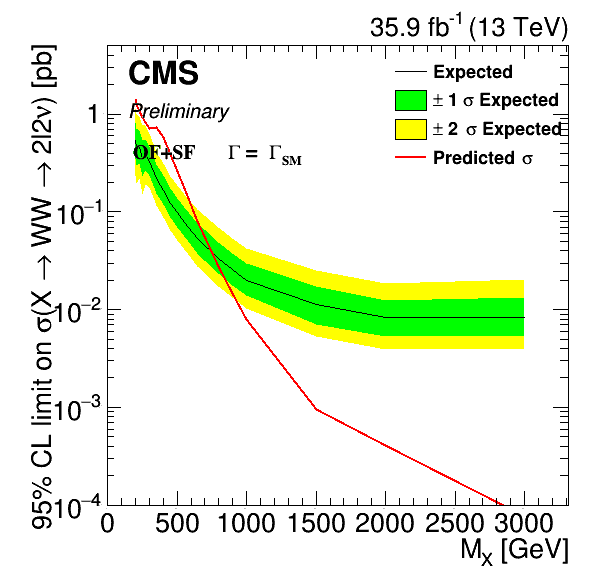
\includegraphics[width=0.45\textwidth]{Figs/Limits_fVBF/c2_fvbf_0.png}
}

\subfigure[$f_{VBF}=1$]{
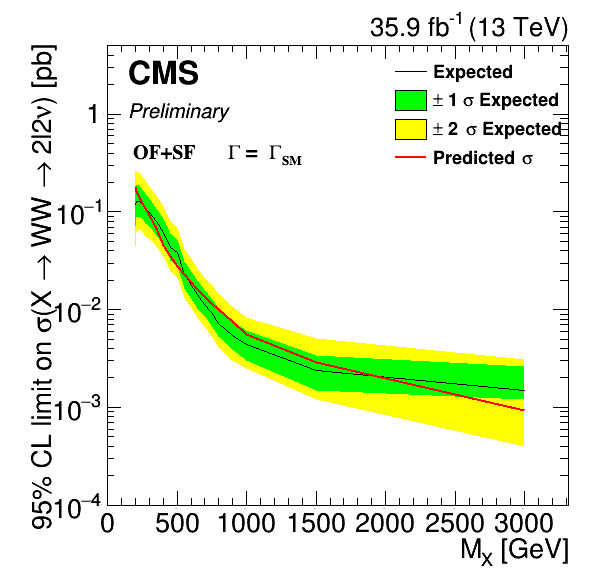
\includegraphics[width=0.45\textwidth]{Figs/Limits_fVBF/c2_fvbf_1.png}
}


\caption{95$\%$ CL exclusion limits,  on the production ggH and VBF cross section times branching for differents $f_{VBF}$ fraction.  The red  line represent the predicted cross-section for EW high mass bosons in  the free floating case (Fig. $a$), only the predicted vector boson cross-section in $f_{VBF}=0$ case (Fig. $b$) 
and only the predicted gluon-gluon fusion cross-section in $f_{VBF}=1$ case (Fig. $c$)  .}
    \label{fig:UL_fvbf}
\end{figure}


\begin{center}
  \begin{tabular}{ l | c |c| r }
    \hline
    Mass                    & 300 GeV & 700 GeV  &  1500 GeV                 \\ \hline     
    Observed Limit  sigma$<$&  0.3334& 0.0457   & 0.0112                    \\\hline
    Expected  2.5\% sigma$<$&  0.1774& 0.0238   & 0.0053                   \\\hline
    Expected 16.0\% sigma$<$&  0.2386& 0.0322   & 0.0071                   \\\hline
    Expected 50.0\% sigma$<$&  0.3340& 0.0454   & 0.0112                   \\\hline
    Expected 84.0\% sigma$<$&  0.4684& 0.0660   & 0.0173                   \\\hline
    Expected 97.5\% sigma$<$&  0.6352& 0.0928   & 0.0249                   \\\hline
    
    \hline
  \end{tabular}

\caption{Upper limits numerical values in free flaoting $f_{VBF}$ case.}
    \label{tab:UL_ff}
\end{center}




\begin{center}
  \begin{tabular}{ l | c |c| r }
    \hline
    Mass                    & 300 GeV & 700 GeV  &  1500 GeV                 \\ \hline     
    Observed Limit  sigma$<$&0.3321  & 0.0458   & 0.0112                    \\\hline
    Expected  2.5\% sigma$<$&0.1764  & 0.0238   & 0.0053                   \\\hline
    Expected 16.0\% sigma$<$&0.2372  & 0.0322   & 0.0071                   \\\hline
    Expected 50.0\% sigma$<$&0.3320  & 0.0454   & 0.0112                   \\\hline
    Expected 84.0\% sigma$<$&0.4657  & 0.0660   & 0.0173                   \\\hline
    Expected 97.5\% sigma$<$&0.6336  & 0.0925   & 0.0249                   \\\hline
    
    \hline
  \end{tabular}

\caption{Upper limits numerical values in $f_{VBF}=0$ case.}
    \label{tab:UL_f0}
\end{center}





\begin{center}
  \begin{tabular}{ l | c |c| r }
    \hline
    Mass                    & 300 GeV & 700 GeV  &  1500 GeV                 \\ \hline     
    Observed Limit  sigma$<$&0.0980  & 0.0003   & 0.0025                    \\\hline
    Expected  2.5\% sigma$<$&0.0533  & 0.0067   & 0.0012                   \\\hline
    Expected 16.0\% sigma$<$&0.0708  & 0.0087   & 0.0015                   \\\hline
    Expected 50.0\% sigma$<$&0.0981  & 0.0112   & 0.0024                   \\\hline
    Expected 84.0\% sigma$<$&0.1369  & 0.0159   & 0.0034                   \\\hline
    Expected 97.5\% sigma$<$&0.1842  & 0.0213   & 0.0051                   \\\hline
    
    \hline
  \end{tabular}

\caption{Upper limits numerical values in $f_{VBF}=0$ case.}
    \label{tab:UL_f1}
\end{center}

\newpage


\subsection{Unblinding}
The expected and observed final limit for  the combination of the opposite and same analysis is shown in fig. \ref{fig:sig_OFSF_comb_un}. 

\begin{figure}[htb]
\centering
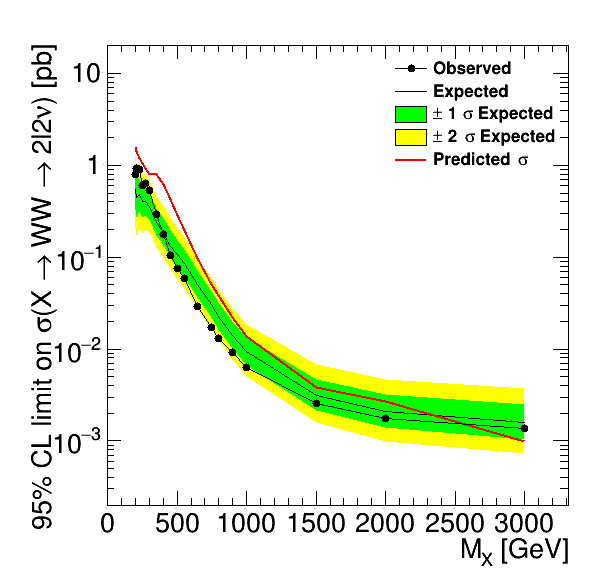
\includegraphics[width=0.65\textwidth]{Figs/unblinding/Limits/c2_FullComb_unbl.png}
\caption{95$\%$ CL exclusion limits,  on the production ggH and VBF cross section times branching fraction as a function of the mass for the { \bf combination} of the two analysis OF and SF, in the full mass range.   The red  line represent the predicted cross-section for EW high mass bosons.}


    \label{fig:sig_OFSF_comb_un}
\end{figure}




The unblinding exlusion limits for the different VFB fration cases are shown in Fig.  \ref{fig:sig_OFSF_comb_un_VBF} 


\begin{figure}[htb]
\centering

\subfigure[Free to floating]{
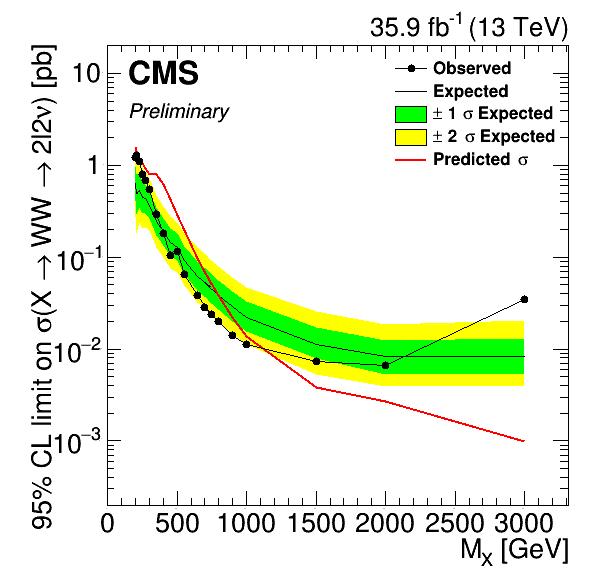
\includegraphics[width=0.45\textwidth]{Figs/unblinding/Limits/c2_floating_unbl.png}
}
\subfigure[$f_{VBF}=0$]{
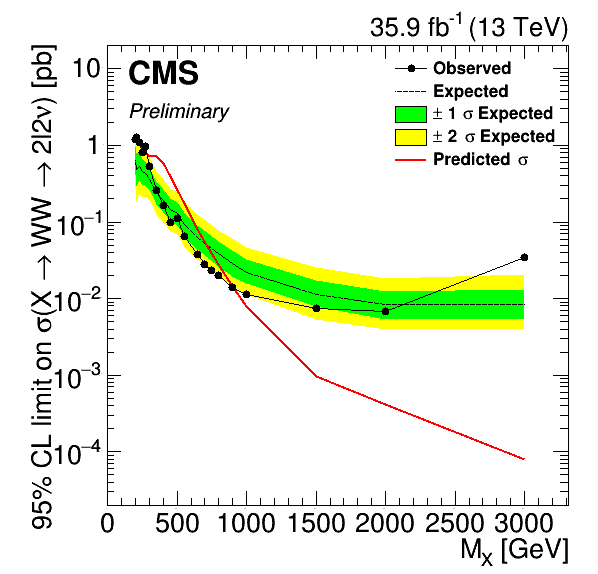
\includegraphics[width=0.45\textwidth]{Figs/unblinding/Limits/c2_fvbf_0_unbl.png}
}

\subfigure[$f_{VBF}=1$]{
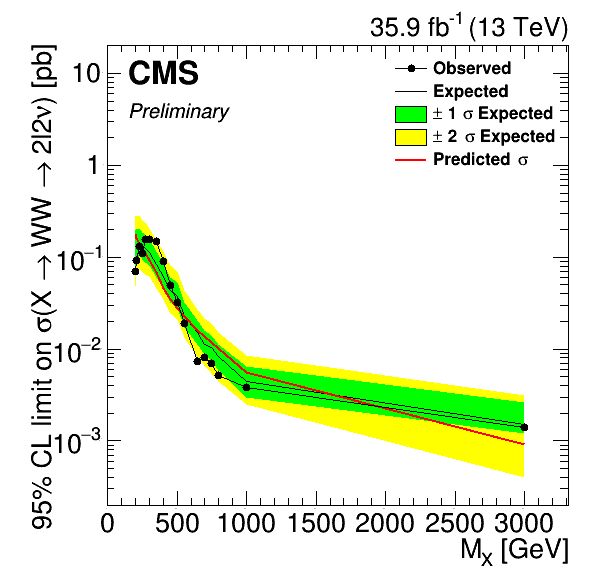
\includegraphics[width=0.45\textwidth]{Figs/unblinding/Limits/c2_unbl_vbf1_BIS.png}

}

\caption{95$\%$ CL observed exclusion limits,  on the production ggH and VBF cross section times branching for differents $f_{VBF}$ fraction.  The red  line represent the predicted cross-section for EW high mass bosons in  the free floating case (Fig. $a$), only the predicted vector boson cross-section in $f_{VBF}=0$ case (Fig. $b$) and only the predicted gluon-gluon fusion cross-section in $f_{VBF}=1$ case (Fig. $c$)  .}    
\label{fig:sig_OFSF_comb_un_VBF}

   \end{figure}

\newpage
\subsection{Goodness of fit}
A goodness of fit test based on the Kolmogorov-Smirnov test statistic has been performed. The
resulting distributions obtained with toys for each individual category, and the value obtained
from a fit to data, are shown in Fig. 115. The p-value in each category is obtained integrating
the test statistic distribution from the value observed in data to infinity, Fig. \ref{fig:GoF_OF_300}, \ref{fig:GoF_OF_2000}, \ref{fig:GoF_SF}. 

\begin{figure}[htb]
\centering
\subfigure[0 jets]{
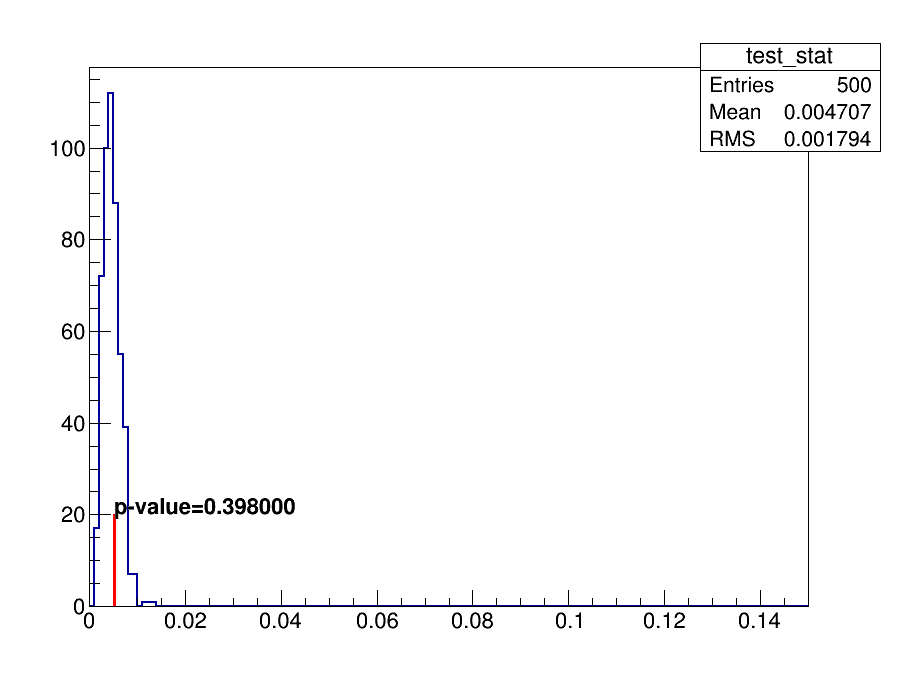
\includegraphics[width=0.45\textwidth]{Figs/unblinding/GoF/pvalue_of0j_300.png}
}
\subfigure[1 jet]{
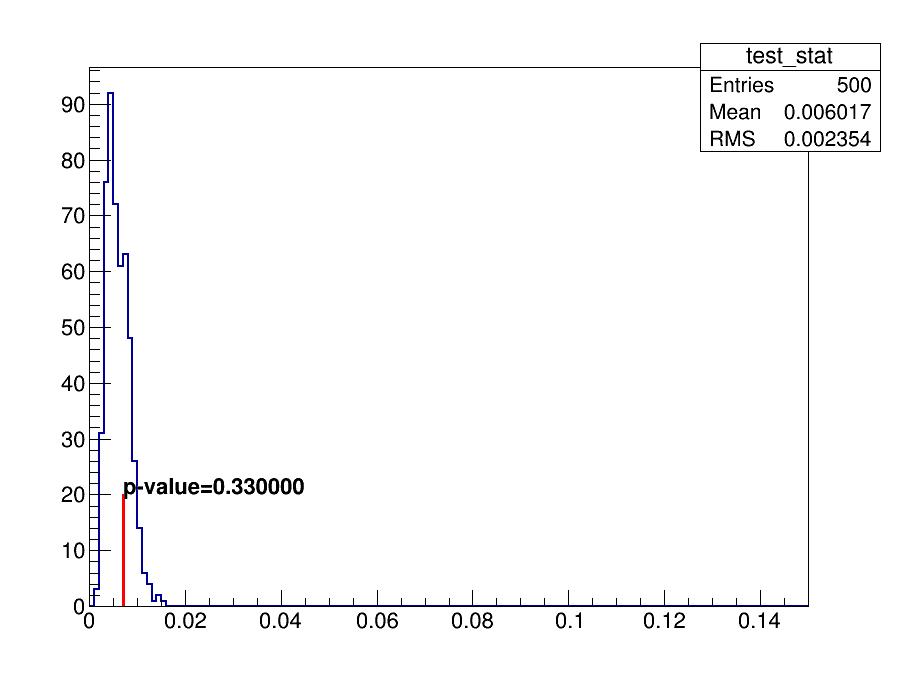
\includegraphics[width=0.45\textwidth]{Figs/unblinding/GoF/pvalue_of1j_300.png}
}
\\
\subfigure[2 jet]{
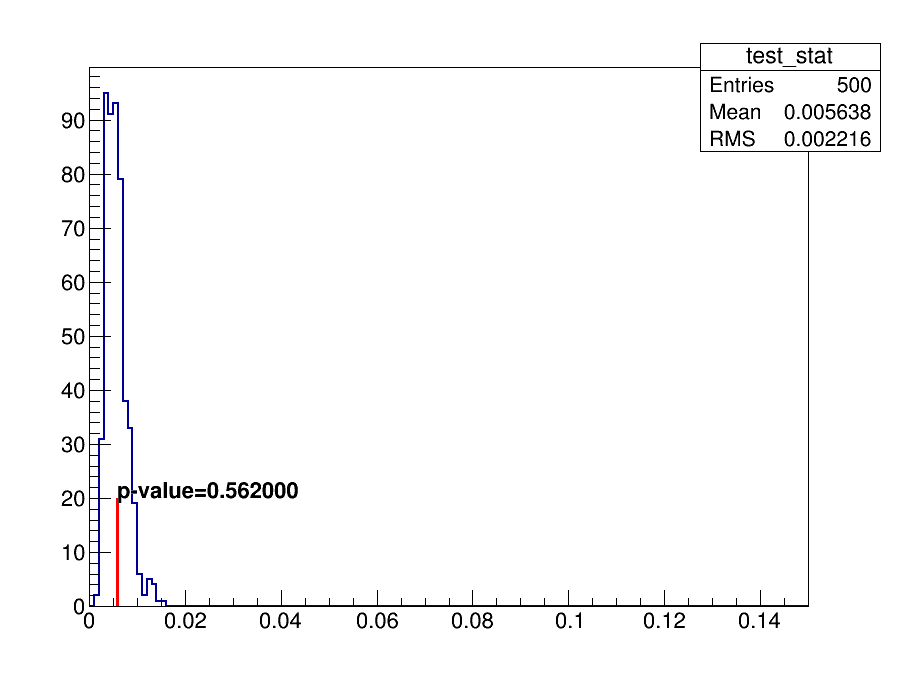
\includegraphics[width=0.45\textwidth]{Figs/unblinding/GoF/pvalue_of2j_300.png}
}
\subfigure[VBF]{
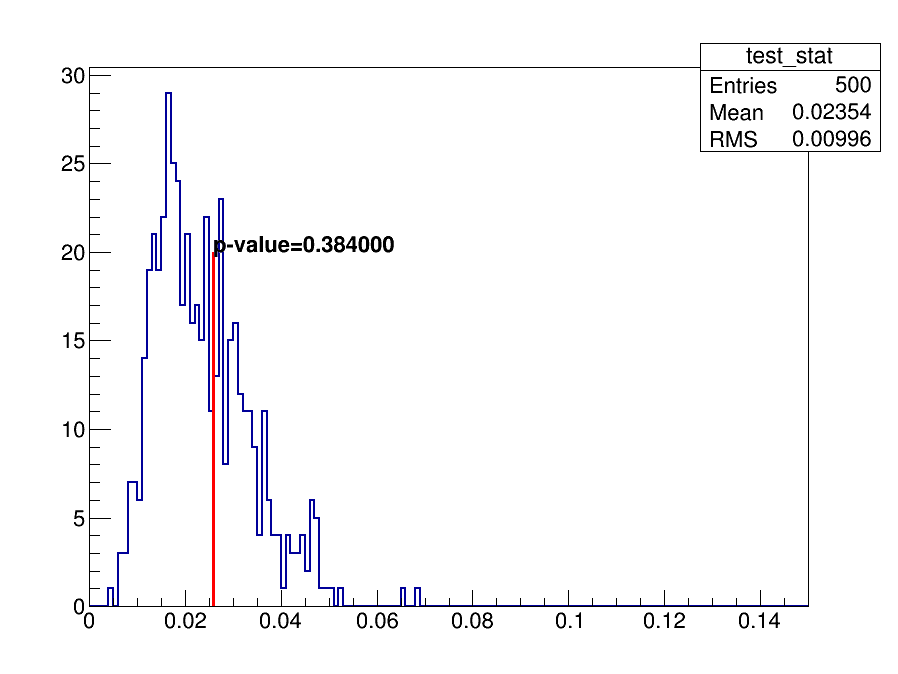
\includegraphics[width=0.45\textwidth]{Figs/unblinding/GoF/pvalue_ofVBF_300.png}
}

\caption{Opposite flavour Kolmogorov-Smirnov goodness of fit results in 0 jets, 1 jet, 2jet and VBF categories for $m_X=$ 300 GeV.}
    \label{fig:GoF_OF_300}
\end{figure}

\newpage
\begin{figure}[htb]
\centering
\subfigure[0 jets]{
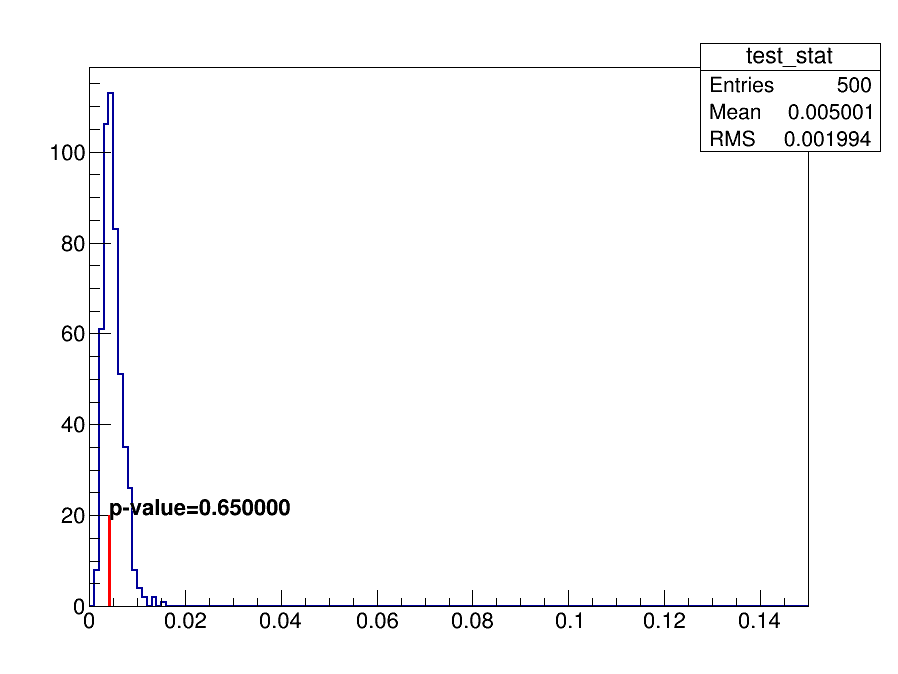
\includegraphics[width=0.45\textwidth]{Figs/unblinding/GoF/pvalue_of0j_2000.png}
}
\subfigure[1 jet]{
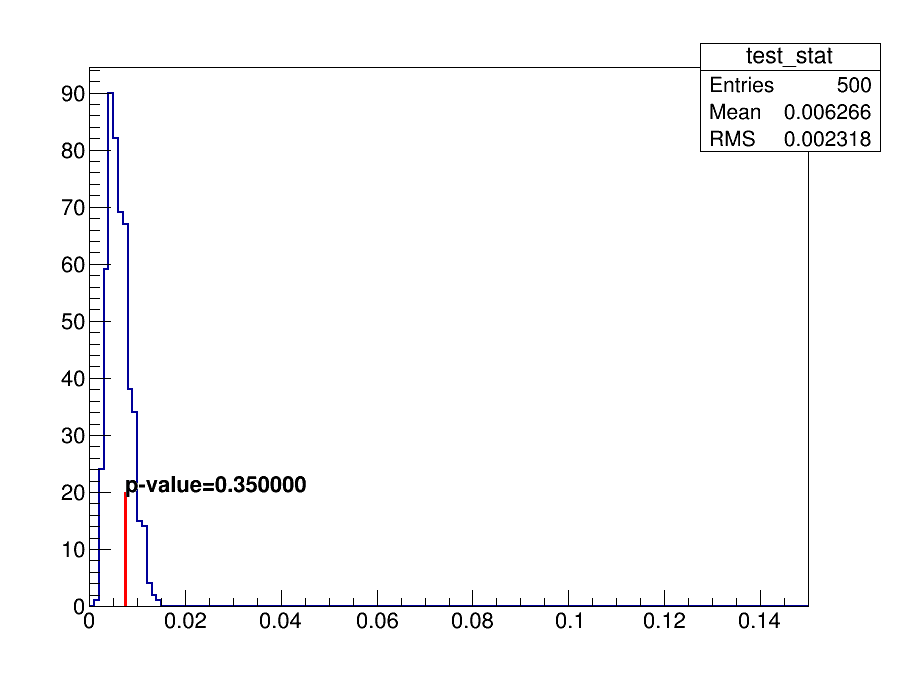
\includegraphics[width=0.45\textwidth]{Figs/unblinding/GoF/pvalue_of1j_2000.png}
}
\\
\subfigure[2 jet]{
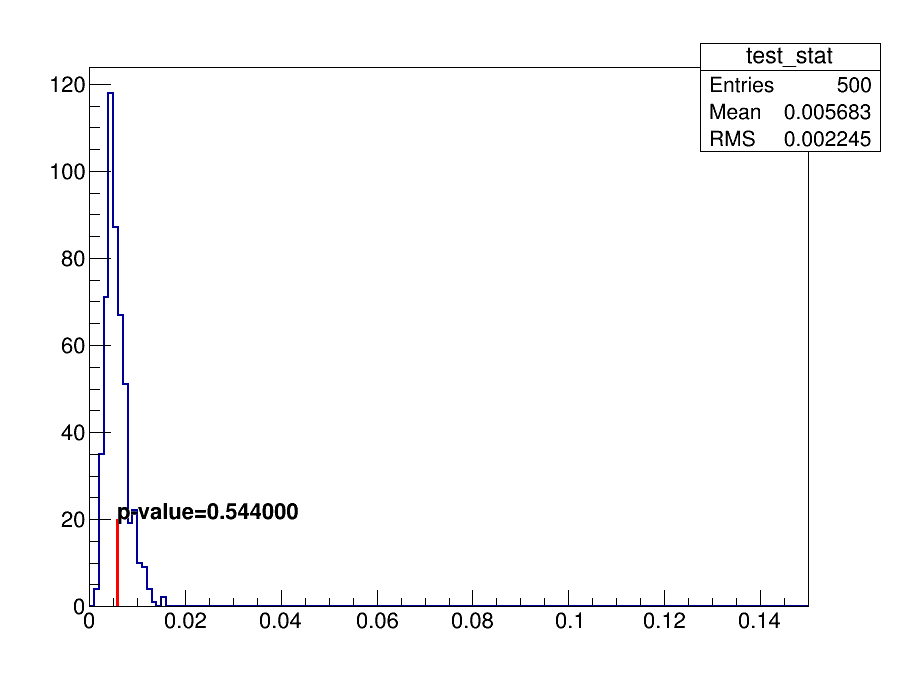
\includegraphics[width=0.45\textwidth]{Figs/unblinding/GoF/pvalue_of2j_2000.png}
}
\subfigure[VBF]{
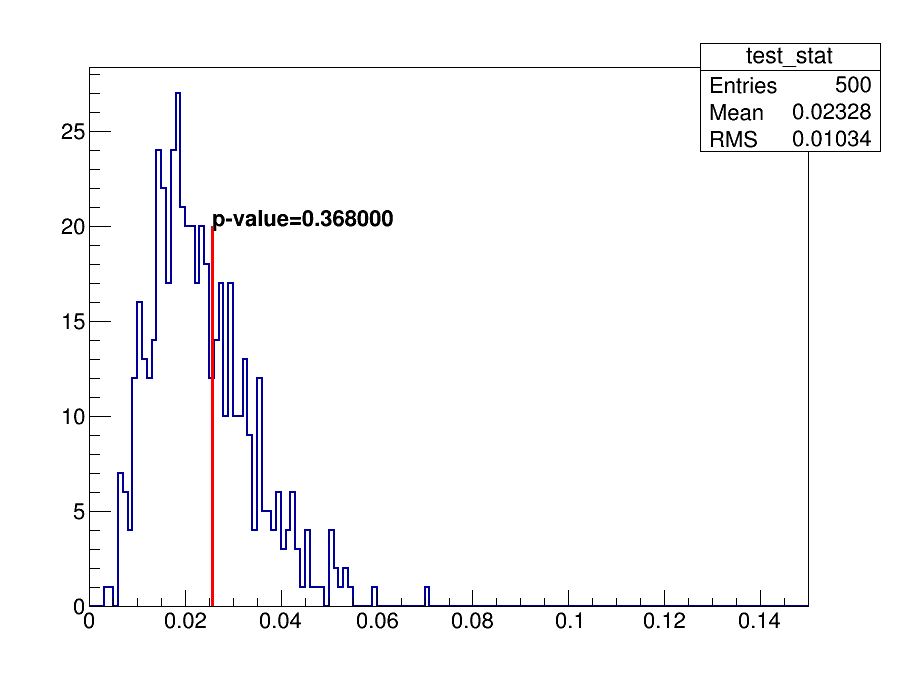
\includegraphics[width=0.45\textwidth]{Figs/unblinding/GoF/pvalue_ofVBF_2000.png}
}

\caption{Opposite flavour Kolmogorov-Smirnov goodness of fit results in 0 jets, 1 jet, 2jet and VBF categories for $m_X=$ 2000 GeV.}
    \label{fig:GoF_OF_2000}
\end{figure}



\newpage
\begin{figure}[htb]
\centering
\subfigure[ee $m_X$=300]{
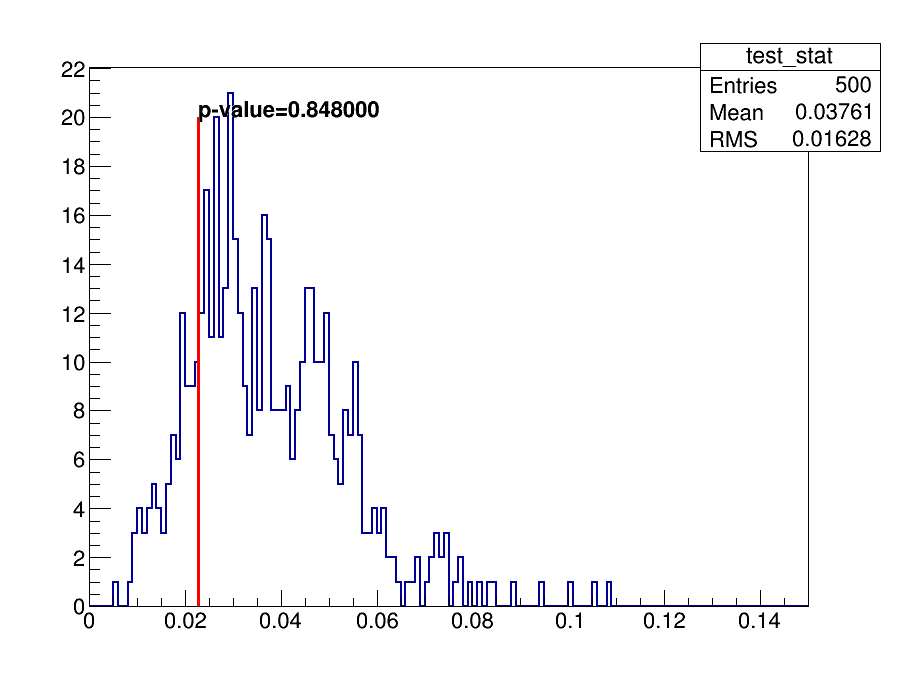
\includegraphics[width=0.45\textwidth]{Figs/unblinding/GoF/pvalue_ee_VBF_300.png}
}
\subfigure[$\mu \mu$ $m_X$=300]{
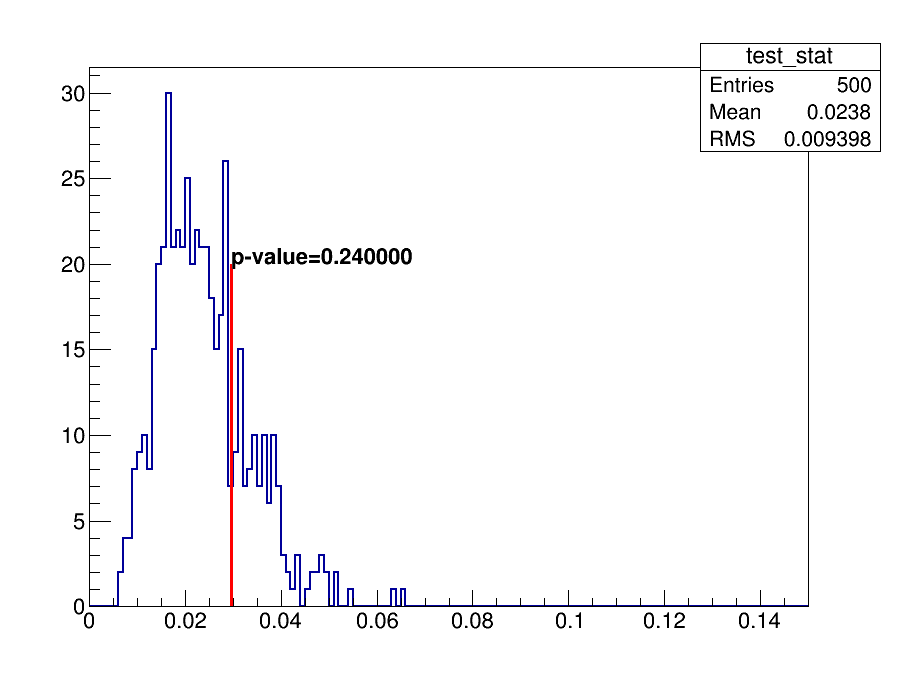
\includegraphics[width=0.45\textwidth]{Figs/unblinding/GoF/pvalue_mm_VBF_300.png}
}
\\
\subfigure[ee $m_X$=2000]{
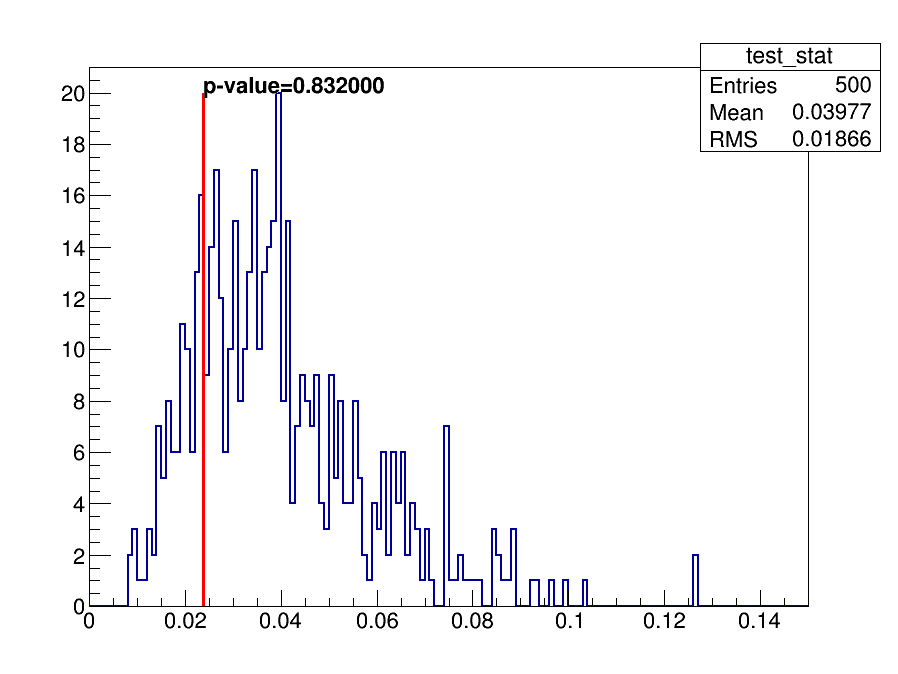
\includegraphics[width=0.45\textwidth]{Figs/unblinding/GoF/pvalue_ee_VBF_2000.png}
}
\subfigure[$\mu \mu$ $m_X$=2000]{
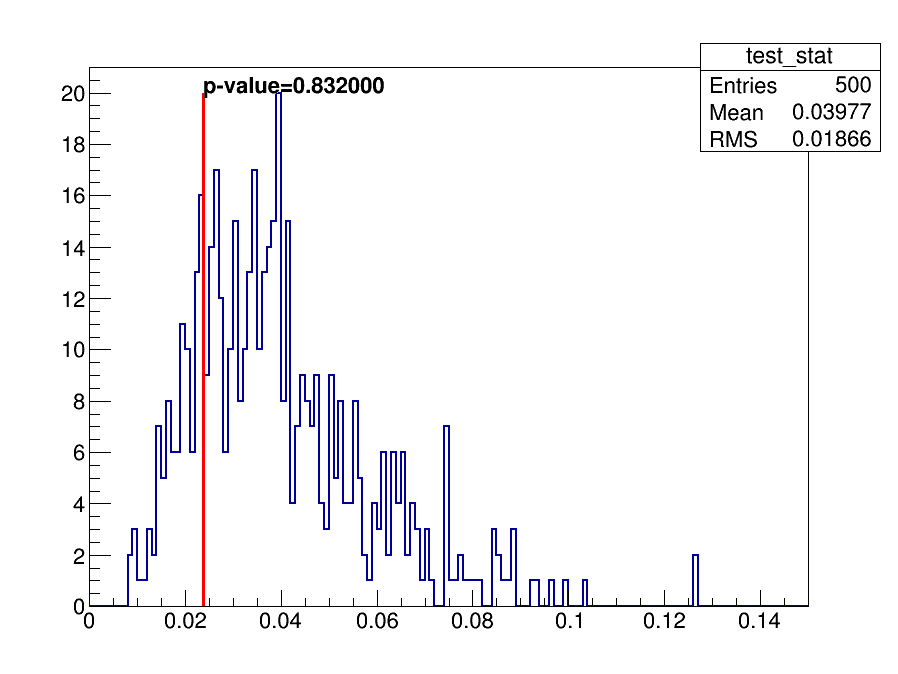
\includegraphics[width=0.45\textwidth]{Figs/unblinding/GoF/pvalue_ee_VBF_2000.png}
}

\caption{Same flavour Kolmogorov-Smirnov goodness of fit results in ee and $\mu \mu$ categories for $m_X=$ 300 GeV and 2000 GeV.}
    \label{fig:GoF_OF_300}
\end{figure}



\newpage
\subsection{Impacts Data Asimov and observed}
The pull of the main nuisance parameters for the combination of all categories, and their impact on the signal strength uncertainty, is shown in Fig. \ref{fig:Impact_dataAsimov} . 
This plot has been obtained performing a fit of the MC Asimov toy. 
The same plot obtained after the fit to data is shown in Fig. \ref{fig:Impact_obs}
\begin{figure}[htb]
\centering
\subfigure[$m_X$=300 GeV, $\mu =0$]{
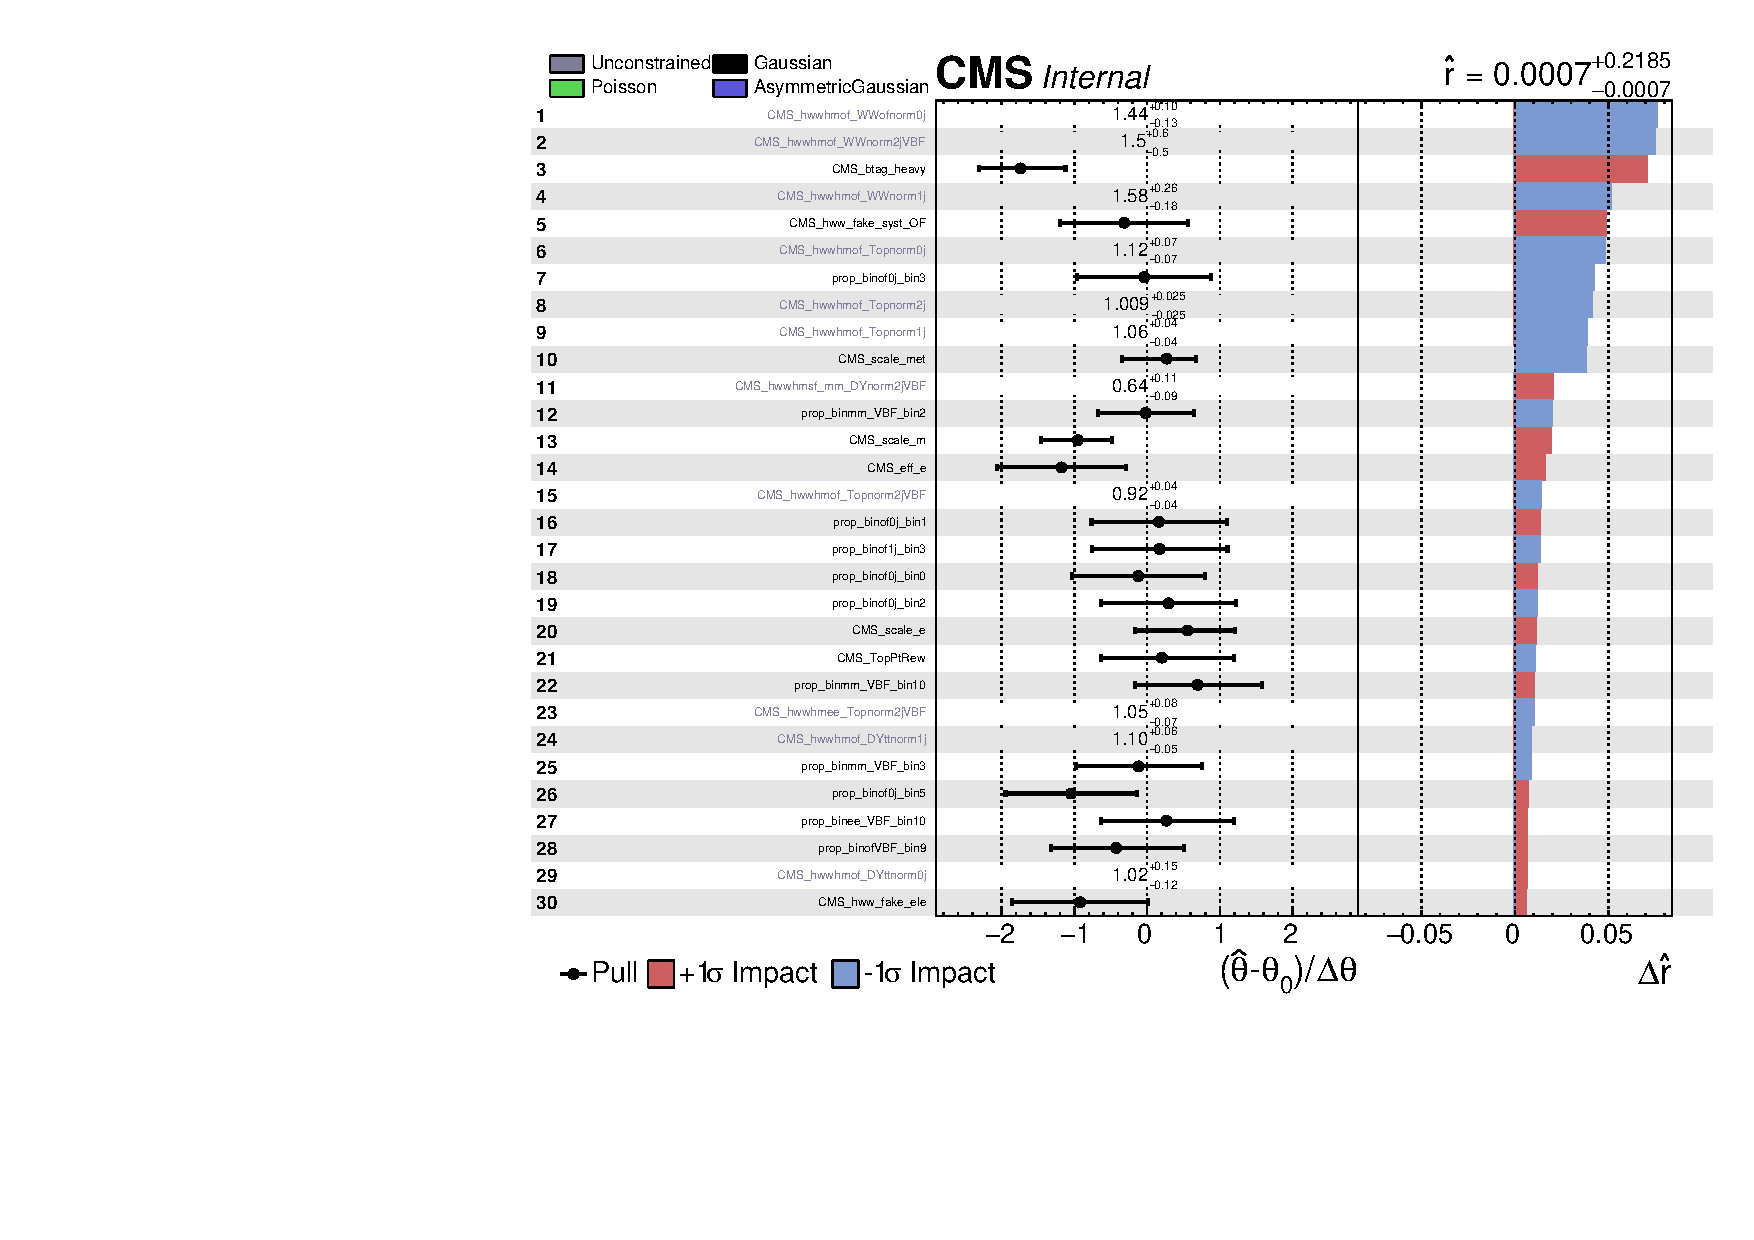
\includegraphics[width=0.5\textwidth]{Figs/unblinding/Impact_dataAsimov/impactsDataAsimov_300_expect0.pdf}
}
\subfigure[$m_X$=300 GeV, $\mu =1$]{
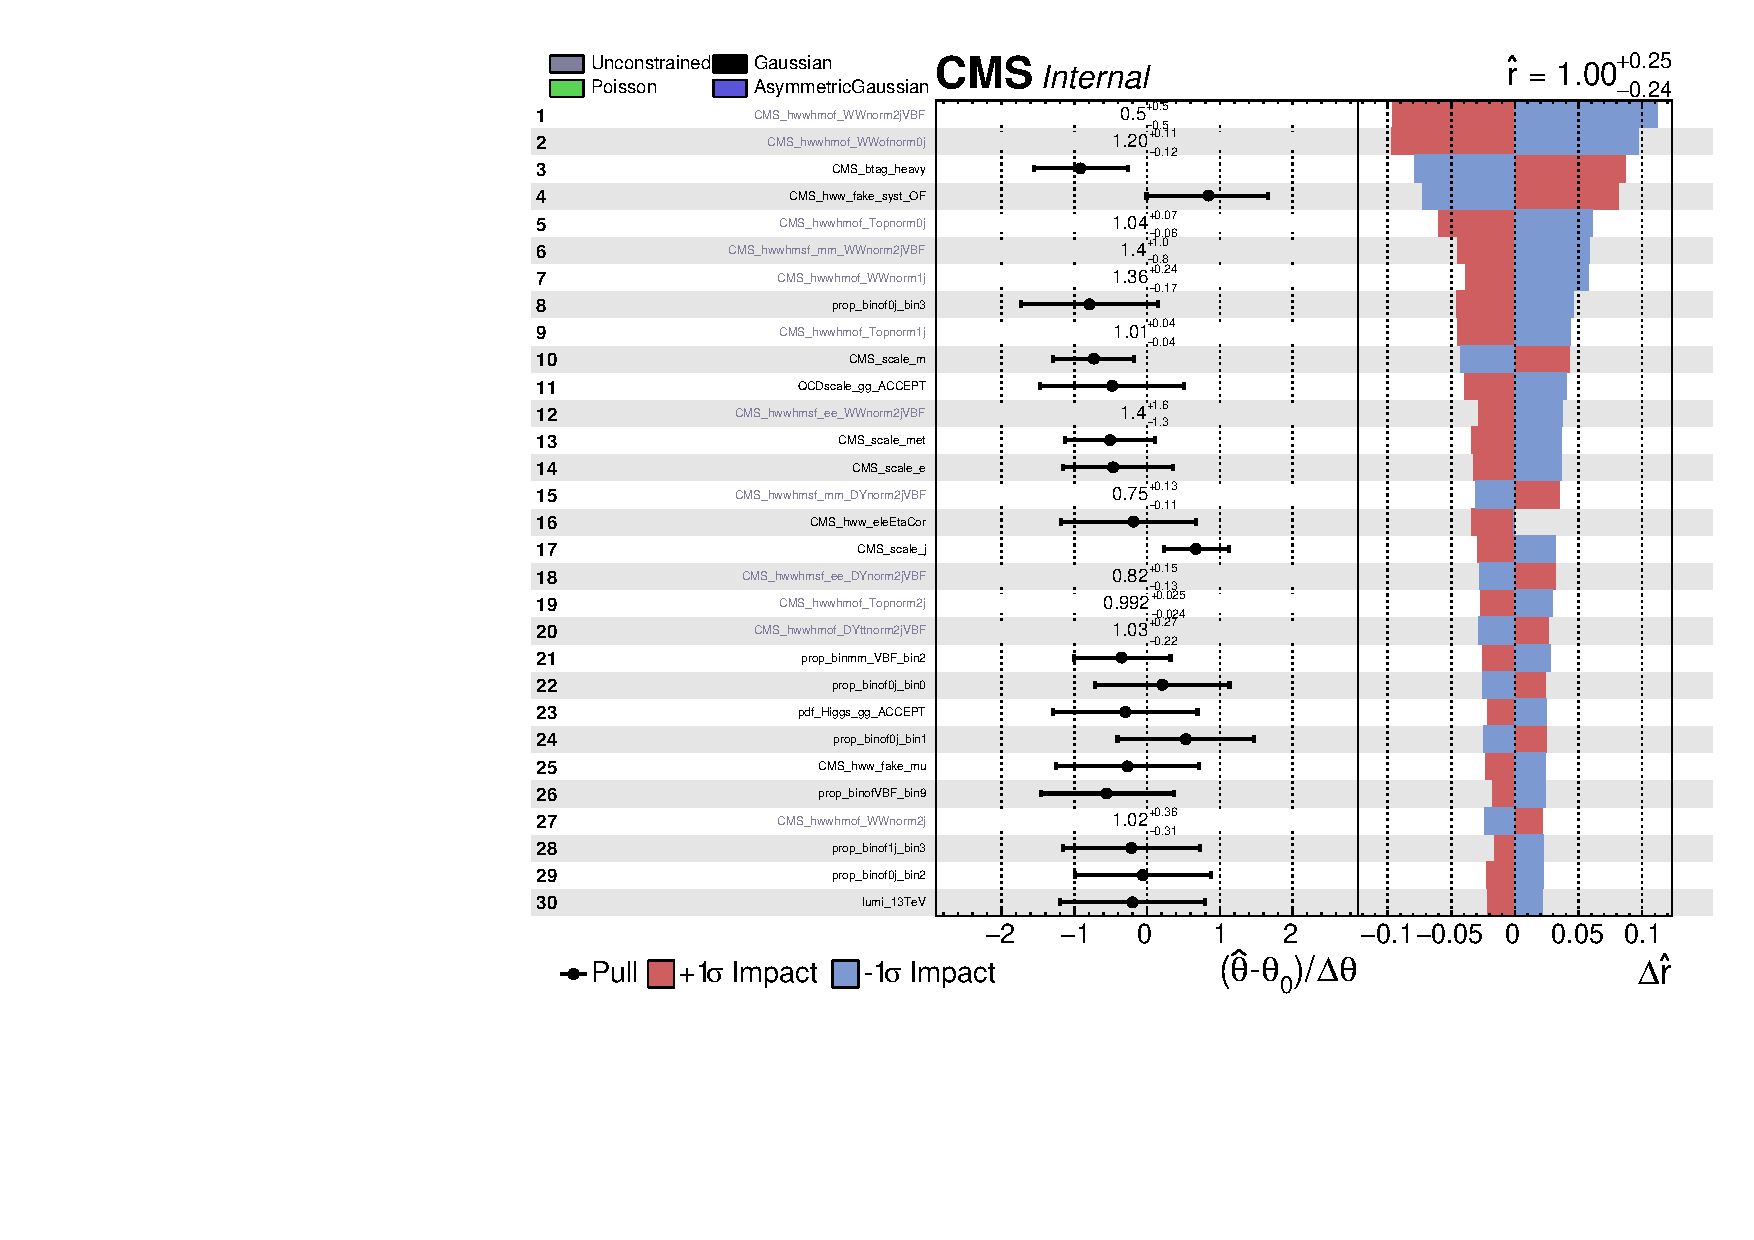
\includegraphics[width=0.5\textwidth]{Figs/unblinding/Impact_dataAsimov/impactsDataAsimov_300_expect1.pdf}
}
\\
\subfigure[$m_X$=2000 GeV, $\mu =0$]{
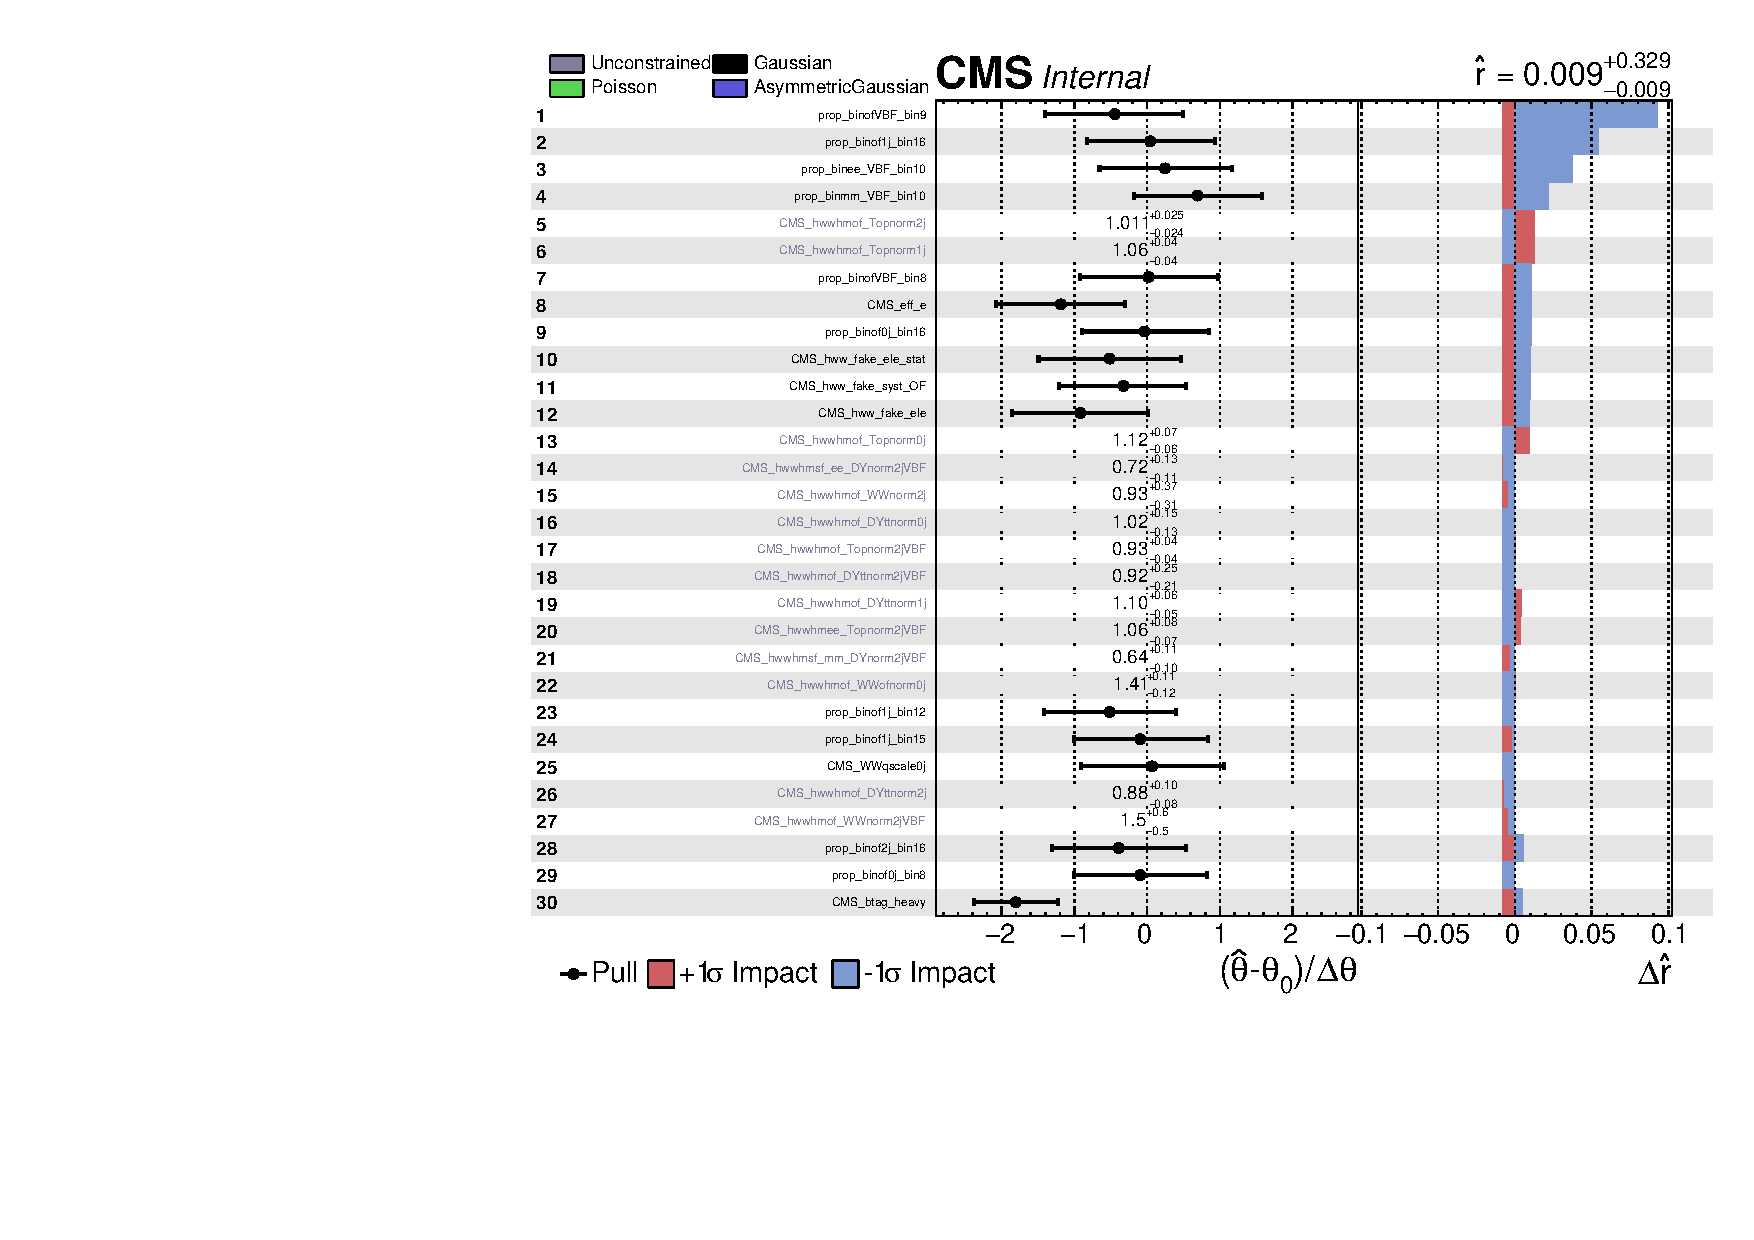
\includegraphics[width=0.5\textwidth]{Figs/unblinding/Impact_dataAsimov/impactsDataAsimov_2000_expect0.pdf}
}
\subfigure[$m_X$=2000 GeV, $\mu =1$]{
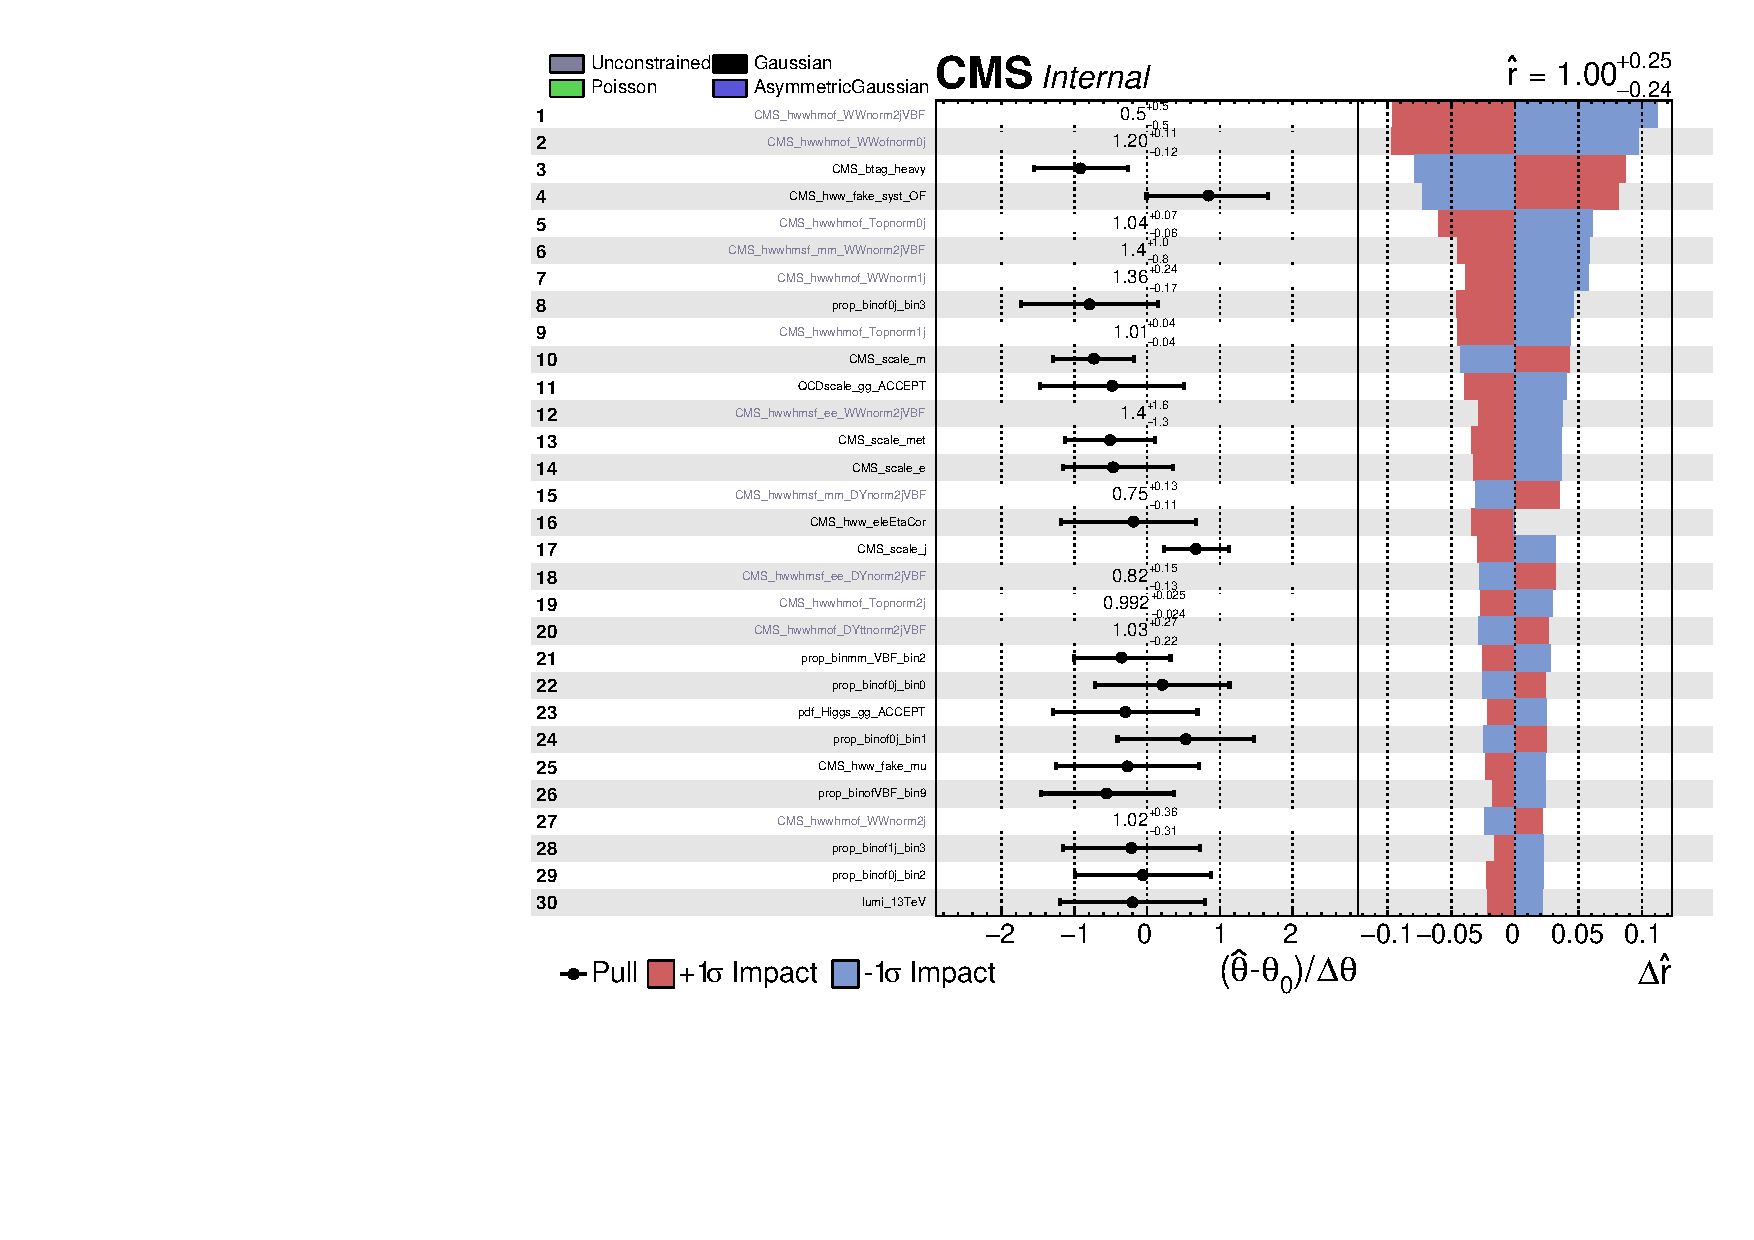
\includegraphics[width=0.5\textwidth]{Figs/unblinding/Impact_dataAsimov/impactsDataAsimov_300_expect1.pdf}
}

\caption{Pull of the 30 main nuisance parameters and their impact on the combined signal strength for the MC Asimov toy for two different mass point, 300 Gev and 2000 GeV, in $\mu=0$ and $\mu=1$ case.}
    \label{fig:Impact_dataAsimov}
\end{figure}



\begin{figure}[htb]
\centering
\subfigure[$m_X$=300 GeV ]{
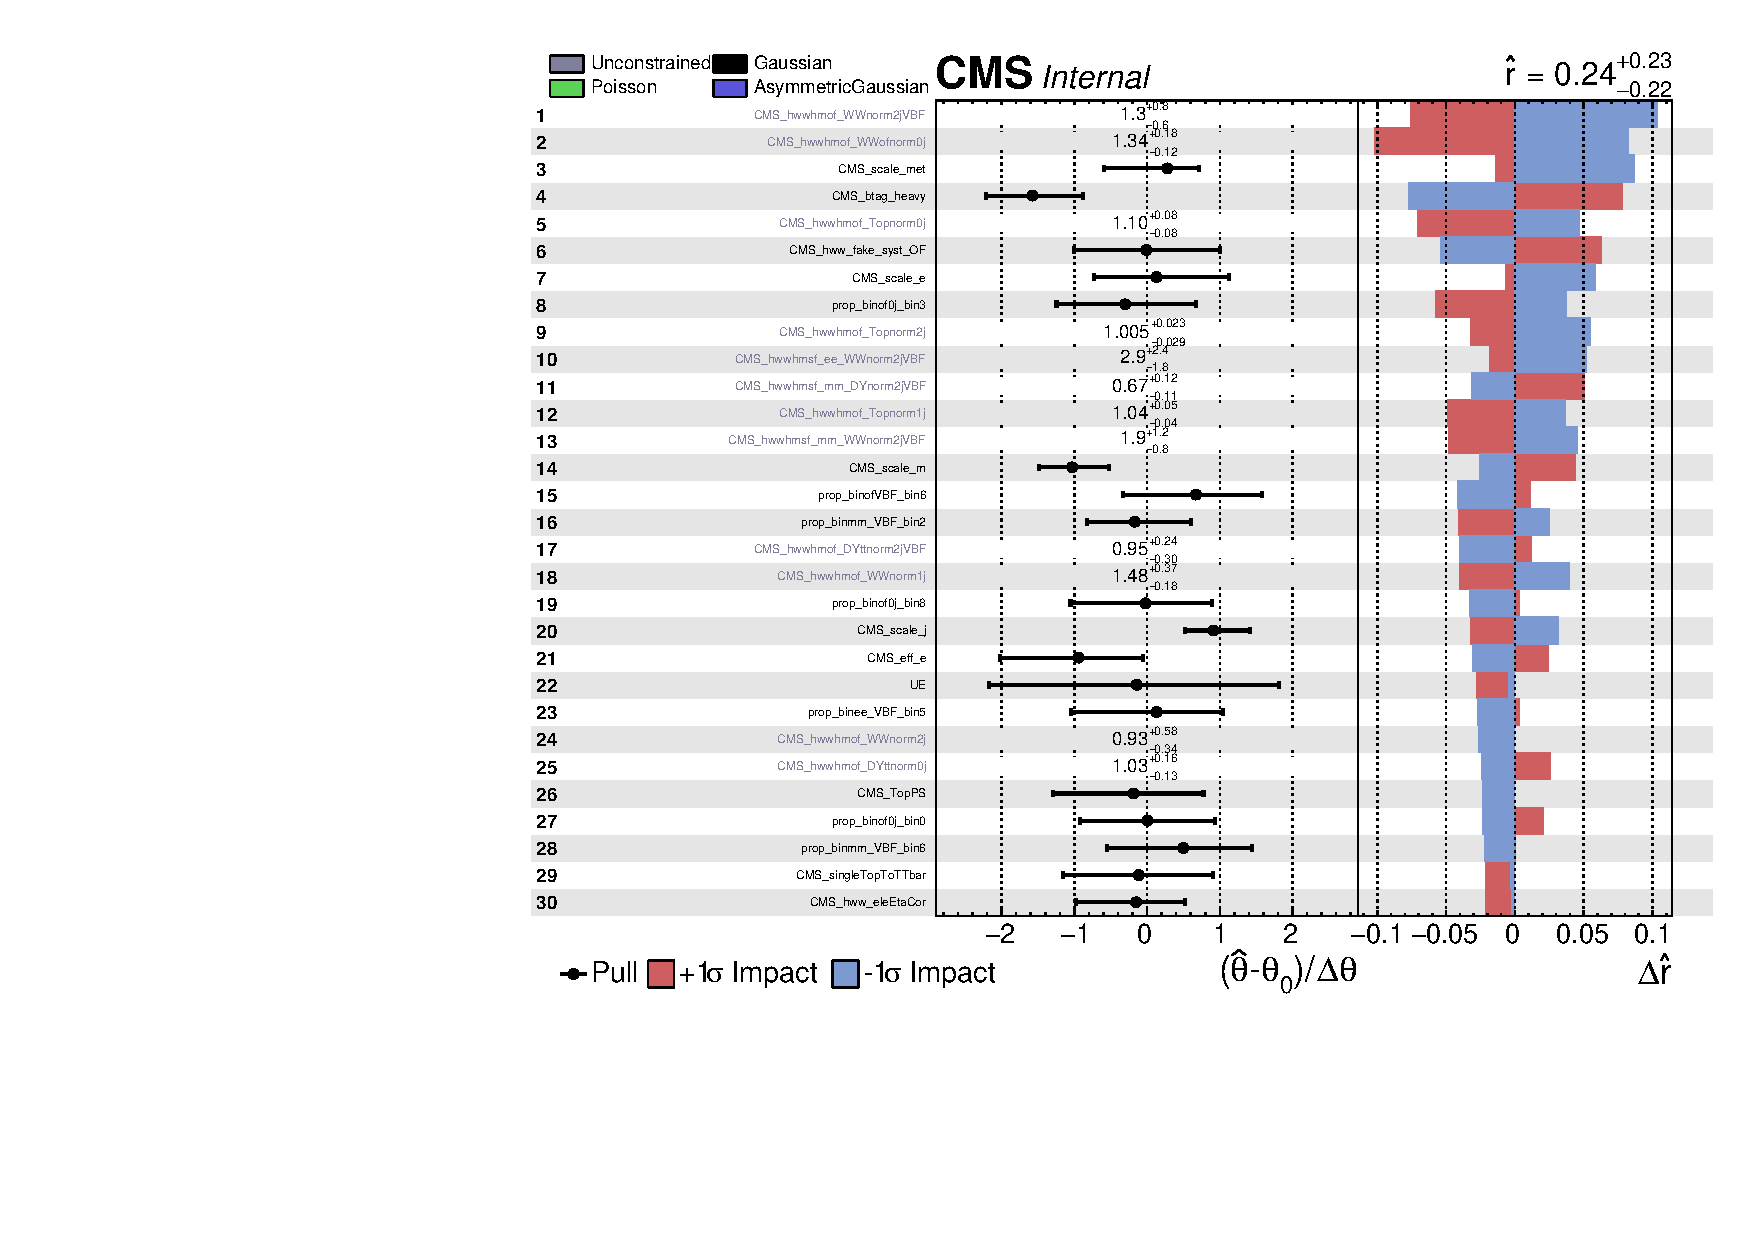
\includegraphics[width=0.5\textwidth]{Figs/unblinding/Impact_obs/impacts300.pdf}
}
\subfigure[$m_X$=2000 GeV]{
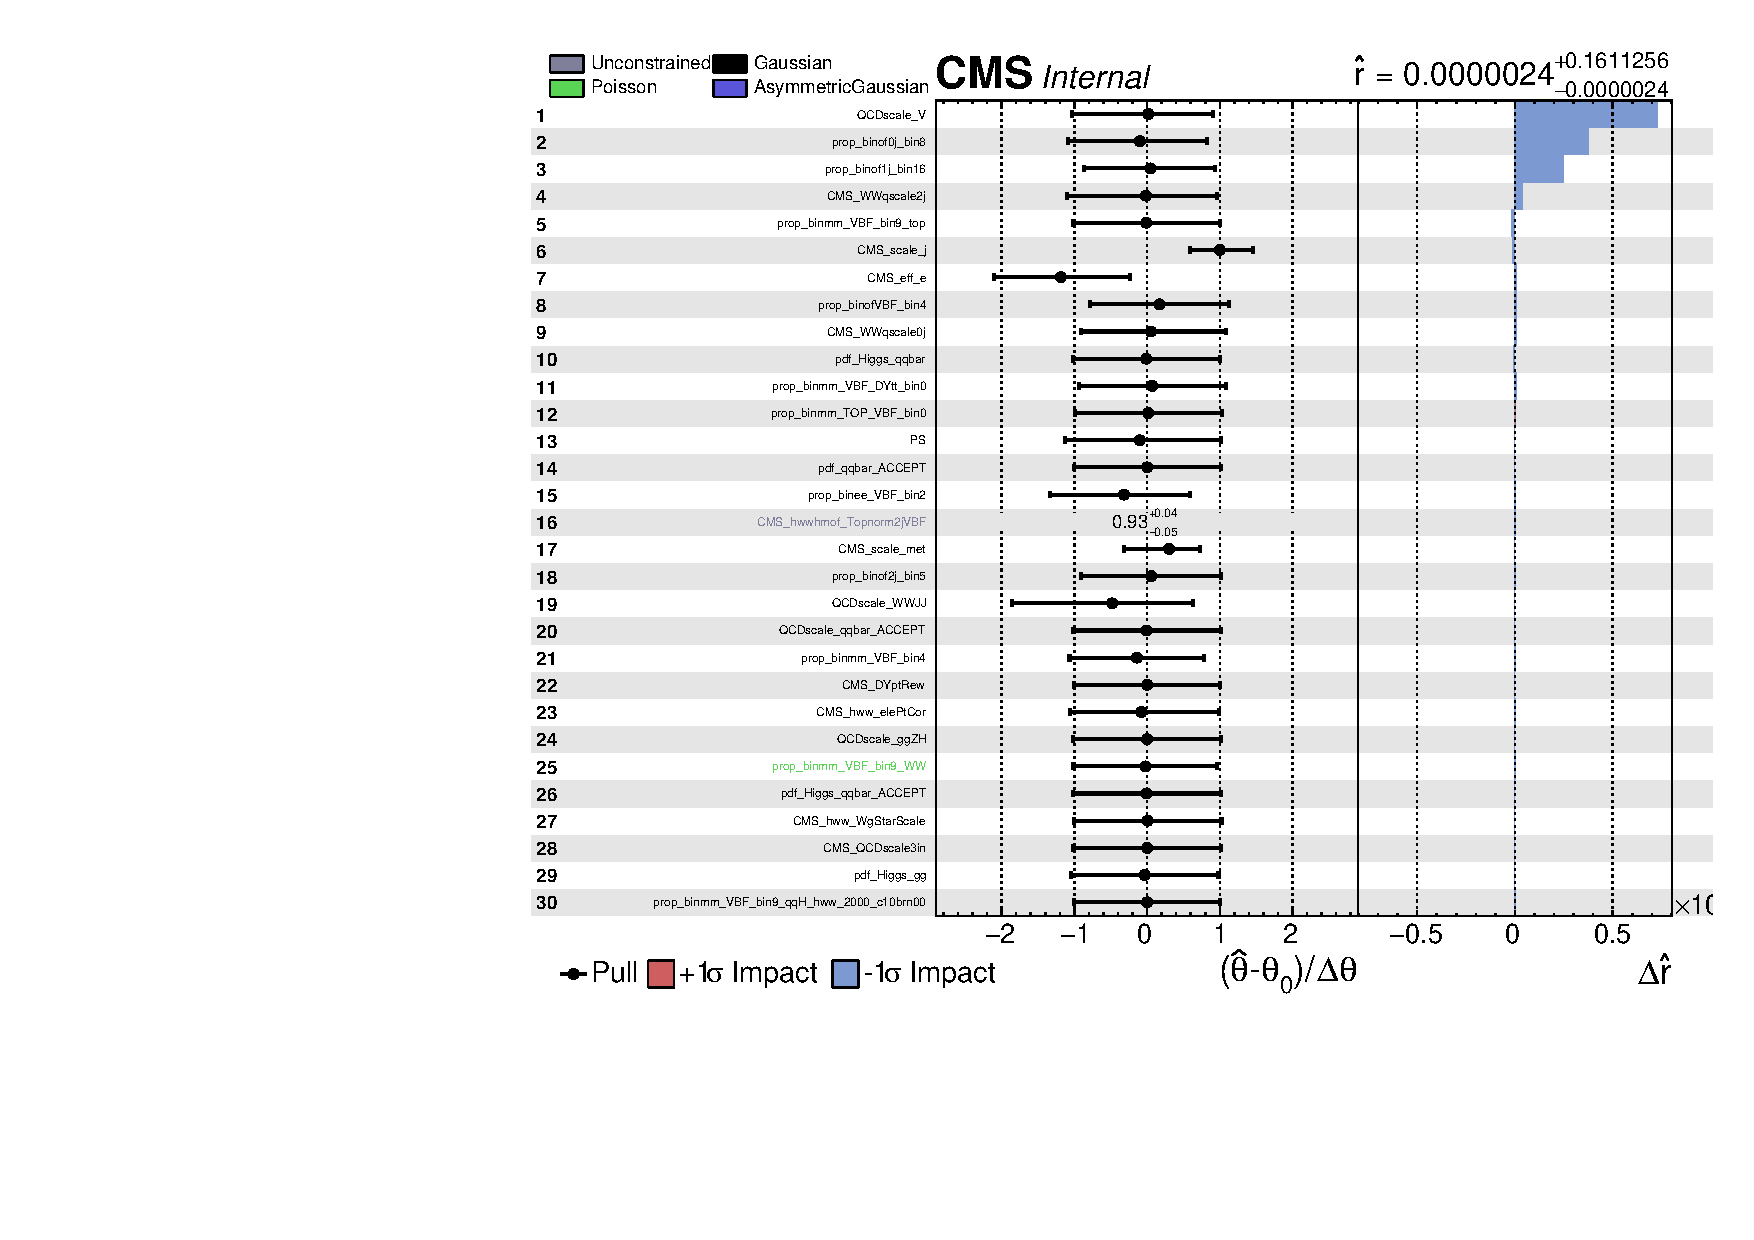
\includegraphics[width=0.5\textwidth]{Figs/unblinding/Impact_obs/impacts2000.pdf}
}

\caption{Pull of the 30 main nuisance parameters and their impact on the combined signal strength for the data for two different mass point, 300 Gev and 2000 GeV.}
    \label{fig:Impact_obs}
\end{figure}



\newpage
\clearpage

\subsection{2HDM results}

In Fig. ~\ref{fig:MSSM} the exclusion limits are shown for the $m_h^{mod+}$ scenario on the left and the hMSSM scenario on the right. The dashed line marks the limit, while the green area shows the side of the limit that is excluded. The bands surrounding the limit indicate the $\pm 1,2\sigma$ contours. For both scenarios the region at low values of $m_{A}$ and $\tan\beta$ is excluded. These results complement well with the exclusion limit given by the MSSM $H\rightarrow\tau\tau$ analysis, where the sensitivity is lower for low $m_{A}$ and $\tan\beta$.

\begin{figure}[htb]
\centering
\subfigure[$m_h^{mod+}$]{
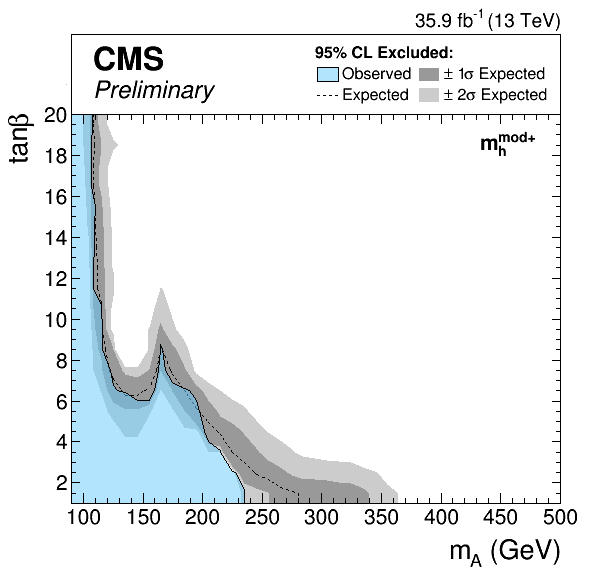
\includegraphics[width=0.45\textwidth]{Figs/unblinding/2HDM/mhmodp.png}
}
\subfigure[hMSSM]{
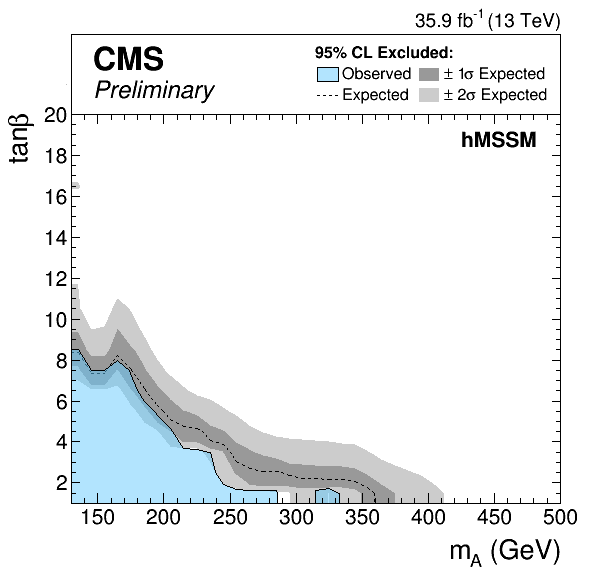
\includegraphics[width=0.45\textwidth]{Figs/unblinding/2HDM/hmssm.png}
}

\caption{95$\%$ CL exclusion limits on the MSSM $m_h^{mod+}$ scenario (left) and the hMSSM scenario (right).}
    \label{fig:MSSM}
\end{figure}

In Fig. ~\ref{fig:2HDM1} and ~\ref{fig:2HDM2} the exclusion limits are shown for a 2HDM. The limits in ~\ref{fig:2HDM1} for both a type-1 and type-2 2HDM is displayed in a $\cos(\beta-\alpha)$-$\tan\beta$ plane, in which the neutral heavy Higgs boson masses are $m_{H}=m_{A}=200$, $300$, $500\,$GeV and the convention $\sin(\beta-\alpha) > 0$ is used. The plots in Fig. ~\ref{fig:2HDM2} show the limit in the $m_{H}$-$\tan\beta$ plane. Here it is again assumed that $m_{H}=m_{A}$ and $\sin(\beta-\alpha) > 0$, but here the relationship between $\beta$ and $\alpha$ is $\cos(\beta-\alpha)=0.1$. The exclusion limits seen here are larger compared to those produced in the similar analysis by ATLAS. A possible reason may be the choice of the discriminating variable $m_{T}^{I}$ or the different categorization.

\begin{figure}[htb]
\centering
\subfigure[Type-1, $m_{H}=200\,$GeV]{
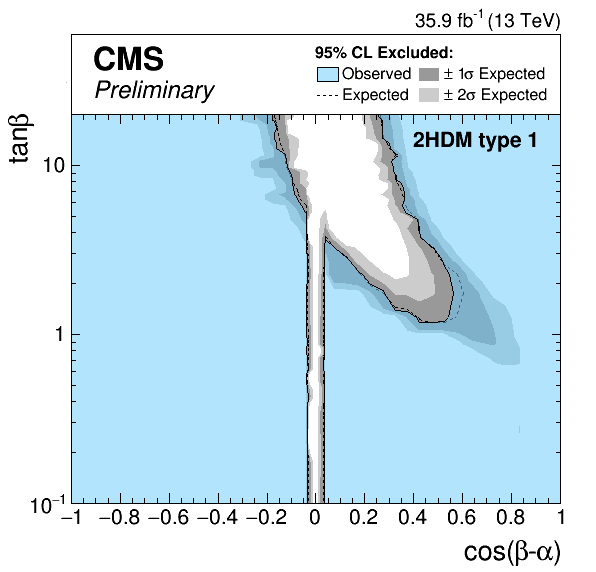
\includegraphics[width=0.45\textwidth]{Figs/unblinding/2HDM/thdm_cosba_t1_200.png}
}
\subfigure[Type-2, $m_{H}=200\,$GeV]{
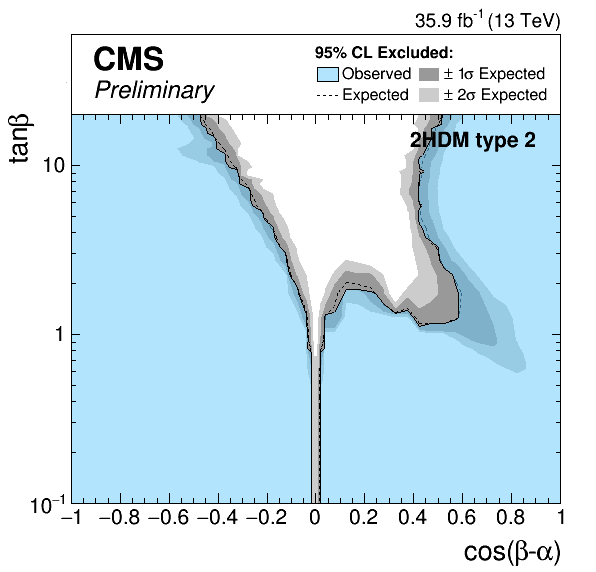
\includegraphics[width=0.45\textwidth]{Figs/unblinding/2HDM/thdm_cosba_t2_200.png}
}
\\
\subfigure[Type-1, $m_{H}=300\,$GeV]{
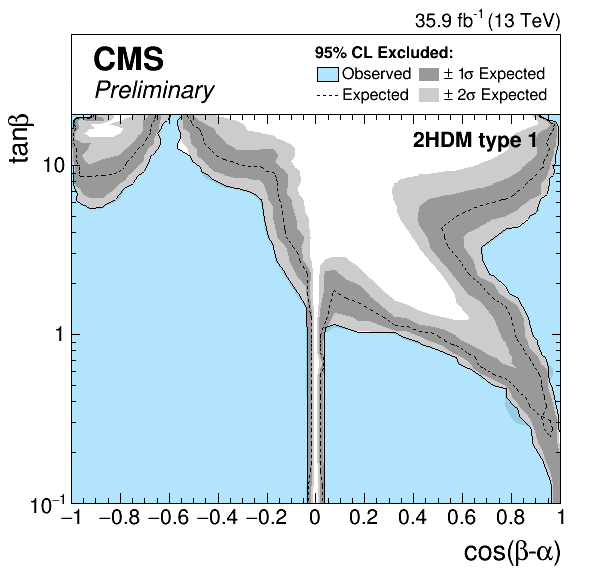
\includegraphics[width=0.45\textwidth]{Figs/unblinding/2HDM/thdm_cosba_t1_300.png}
}
\subfigure[Type-2, $m_{H}=300\,$GeV]{
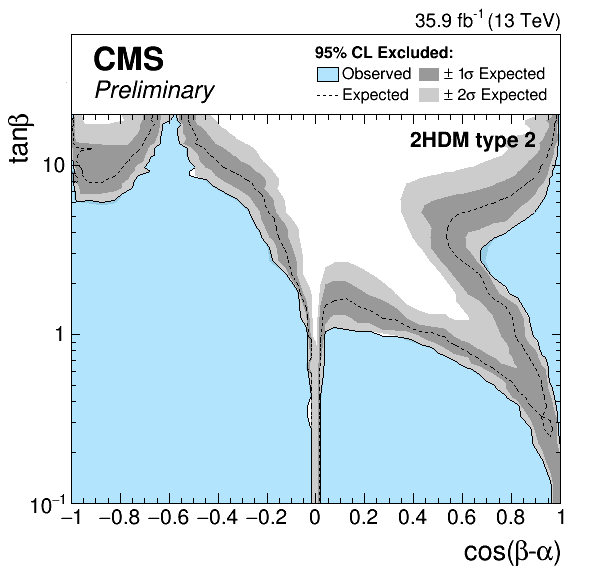
\includegraphics[width=0.45\textwidth]{Figs/unblinding/2HDM/thdm_cosba_t2_300.png}
}
\\
\subfigure[Type-1, $m_{H}=500\,$GeV]{
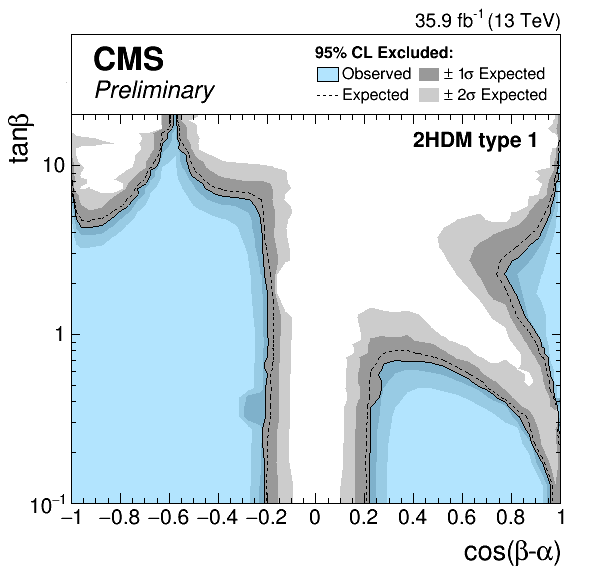
\includegraphics[width=0.45\textwidth]{Figs/unblinding/2HDM/thdm_cosba_t1_500.png}
}
\subfigure[Type-2, $m_{H}=500\,$GeV]{
\includegraphics[width=0.45\textwidth]{Figs/unblinding/2HDM/thdm_cosba_t2_500.png}
}
\caption{95$\%$ CL exclusion limits on a 2HDM with $\cos(\beta-\alpha)$ on the x-axis. Limits are shown for a type-1 and type-2 2HDM for different masses $m_{H}=200$, $300$, $500\,$GeV.}
    \label{fig:2HDM1}
\end{figure}

\begin{figure}[htb]
\centering
\subfigure[Type-1, $\cos(\beta-\alpha)=0.1$]{
\includegraphics[width=0.45\textwidth]{Figs/unblinding/2HDM/thdm_mh_t1.png}
}
\subfigure[Type-2, $\cos(\beta-\alpha)=0.1$]{
\includegraphics[width=0.45\textwidth]{Figs/unblinding/2HDM/thdm_mh_t2.png}
}

\caption{95$\%$ CL exclusion limits on a 2HDM with $m_{H}$ on the x-axis. Limits are shown for a type-1 and type-2 2HDM for $\cos(\beta-\alpha)=0.1$.}
    \label{fig:2HDM2}
\end{figure}

